\documentclass[11pt,a4paper]{article}

% Multilingual support - requires XeLaTeX or LuaLaTeX
\usepackage{fontspec}
\usepackage{xeCJK}  % Better Chinese font support, especially for Overleaf
\usepackage{polyglossia}
\setdefaultlanguage{english}
\setotherlanguages{chinese,german}

% Chinese font setup for Overleaf using xeCJK
% IMPORTANT: Overleaf may not have Chinese fonts installed by default
% If you get font errors, try the options below in order, or comment out all font lines

% Option 1: Try Noto Sans CJK SC first (comment out if it doesn't work)
% \setCJKmainfont{Noto Sans CJK SC}
% \setCJKsansfont{Noto Sans CJK SC}

% Option 2: If Noto doesn't work, try Source Han Sans SC
% \setCJKmainfont{Source Han Sans SC}
% \setCJKsansfont{Source Han Sans SC}

% Option 3: If fonts still don't work, comment out all \setCJK* lines above
% The document will compile but Chinese text may not display correctly

% Page layout
\usepackage[top=2.5cm,bottom=2.5cm,left=3cm,right=2.5cm]{geometry}
\usepackage{fancyhdr}
\setlength{\headheight}{27pt}
\pagestyle{fancy}
\fancyhf{}
\fancyhead[C]{WeChat Europe Analysis / 微信欧洲分析 / WeChat Europa-Analyse}
\fancyfoot[C]{\thepage}

% Hyperlinks
\usepackage{hyperref}
\hypersetup{
    colorlinks=true,
    linkcolor=blue,
    filecolor=magenta,      
    urlcolor=cyan,
    pdftitle={Why WeChat's Ecosystem Model Hasn't Become Popular in Europe},
    pdfauthor={Germany Startup Map Platform}
}

% Graphics and diagrams
\usepackage{graphicx}
\usepackage{tikz}
\usetikzlibrary{shapes,arrows,positioning,calc,decorations.pathreplacing,shapes.geometric,fit,backgrounds,matrix}

% Title
\title{\textbf{为什么微信生态这种产品思路没有在欧洲流行起来}\\
\large Why WeChat's Ecosystem Model Hasn't Become Popular in Europe\\
\large Warum WeChats Ökosystem-Modell in Europa nicht populär wurde}
\author{Germany Startup Map Platform}
\date{\today}

\begin{document}

\maketitle

\section{执行摘要 / Executive Summary / Zusammenfassung}

微信作为"超级应用"（Super App）在中国取得了巨大成功，将社交、支付、电商、生活服务等整合在一个平台内。然而，这种生态模式在欧洲市场并未获得同样的成功。本文档深入分析导致这一现象的根本原因。

WeChat has achieved tremendous success in China as a "Super App," integrating social networking, payments, e-commerce, and lifestyle services within a single platform. However, this ecosystem model has not achieved similar success in the European market. This document provides an in-depth analysis of the fundamental reasons behind this phenomenon.

WeChat hat in China als "Super-App" großen Erfolg erzielt und soziale Netzwerke, Zahlungen, E-Commerce und Lifestyle-Dienste in einer einzigen Plattform integriert. Dieses Ökosystemmodell hat jedoch auf dem europäischen Markt keinen ähnlichen Erfolg erzielt. Dieses Dokument bietet eine eingehende Analyse der grundlegenden Gründe für dieses Phänomen.

\begin{figure}[ht]
\centering
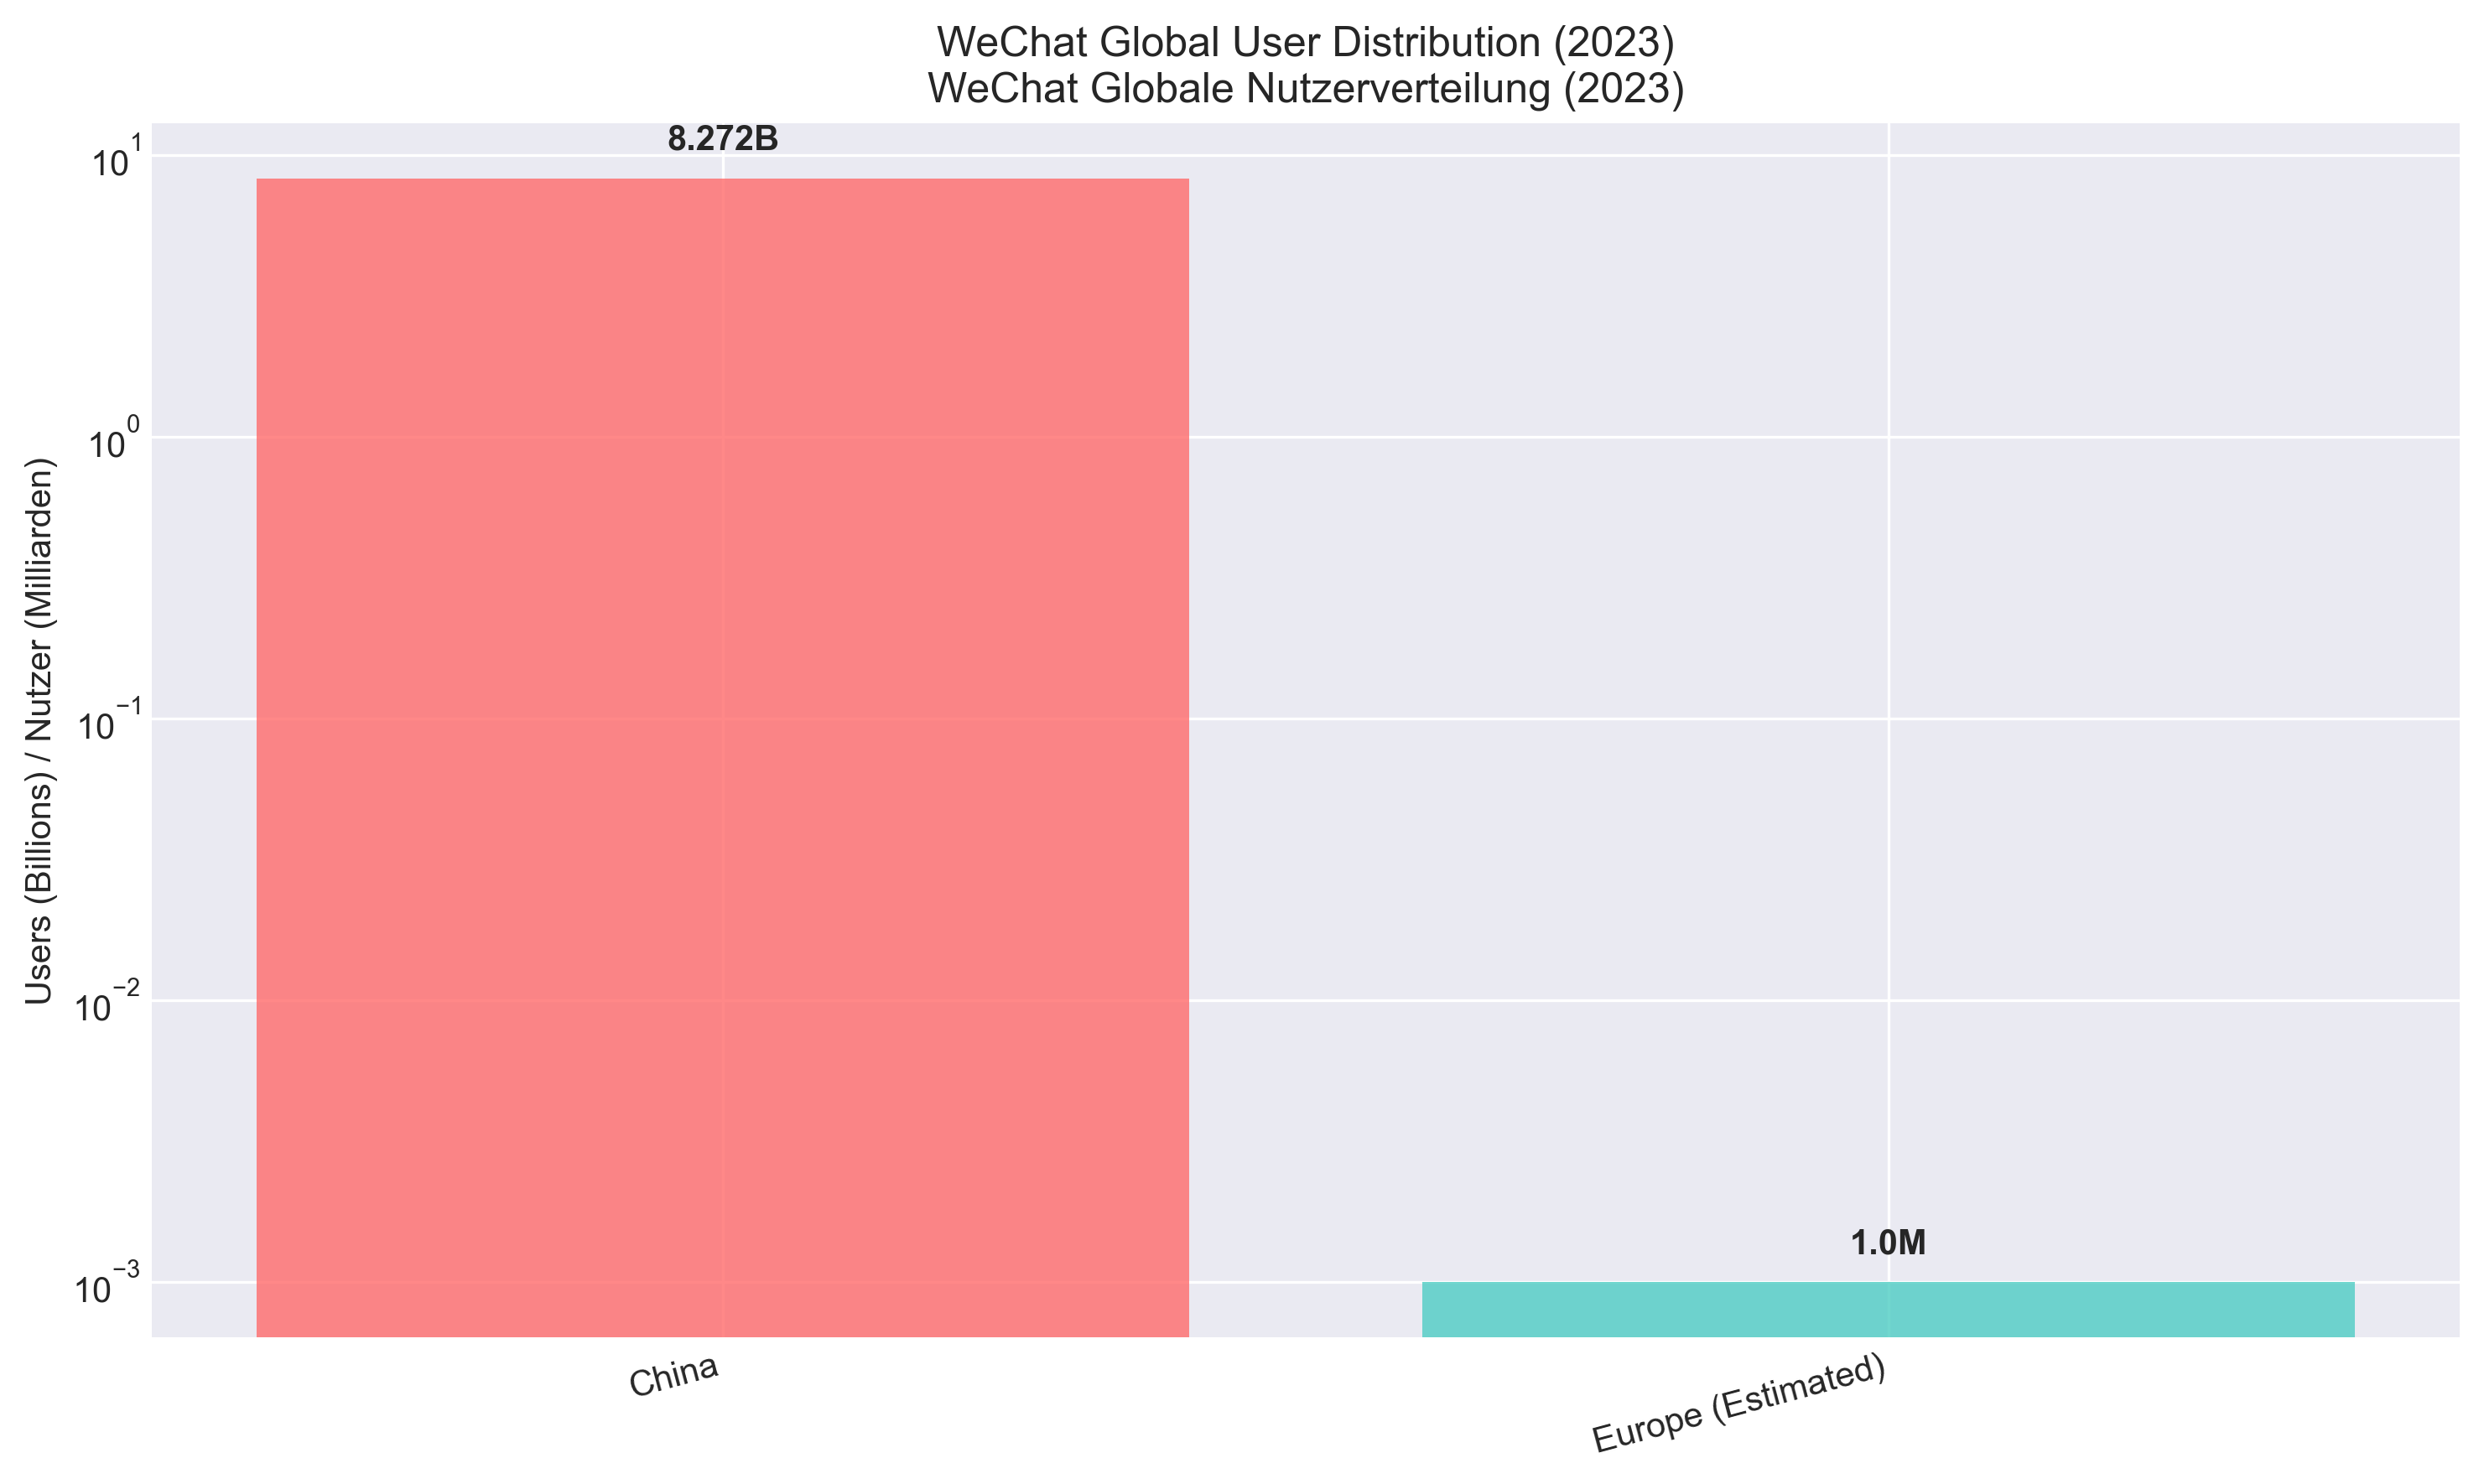
\includegraphics[width=0.9\textwidth]{figures/wechat_global_distribution.png}
\caption{WeChat Global User Distribution (2023) / WeChat Globale Nutzerverteilung (2023)}
\label{fig:wechat-global}
\end{figure}

如图~\ref{fig:wechat-global}所示，WeChat在全球拥有13亿用户，其中8.272亿在中国，而欧洲用户数仅约100万，占全球用户的0.008\%，这清楚地说明了WeChat在欧洲市场的极低渗透率。

As shown in Figure~\ref{fig:wechat-global}, WeChat has 1.3 billion global users, with 827.2 million in China, while European users number only approximately 1 million, accounting for 0.008\% of global users, clearly demonstrating WeChat's extremely low penetration in the European market.

Wie in Abbildung~\ref{fig:wechat-global} dargestellt, hat WeChat weltweit 1,3 Milliarden Nutzer, davon 827,2 Millionen in China, während die europäischen Nutzer nur etwa 1 Million betragen, was 0,008\% der globalen Nutzer ausmacht und deutlich WeChats extrem niedrige Durchdringung auf dem europäischen Markt zeigt.

\section{监管环境差异 / Regulatory Environment Differences / Unterschiede im regulatorischen Umfeld}

\subsection{GDPR与数据保护法规 / GDPR and Data Protection Regulations / DSGVO und Datenschutzbestimmungen}

\textbf{欧洲的严格数据保护要求 / Europe's Strict Data Protection Requirements / Europas strenge Datenschutzanforderungen}

\begin{figure}[ht]
\centering
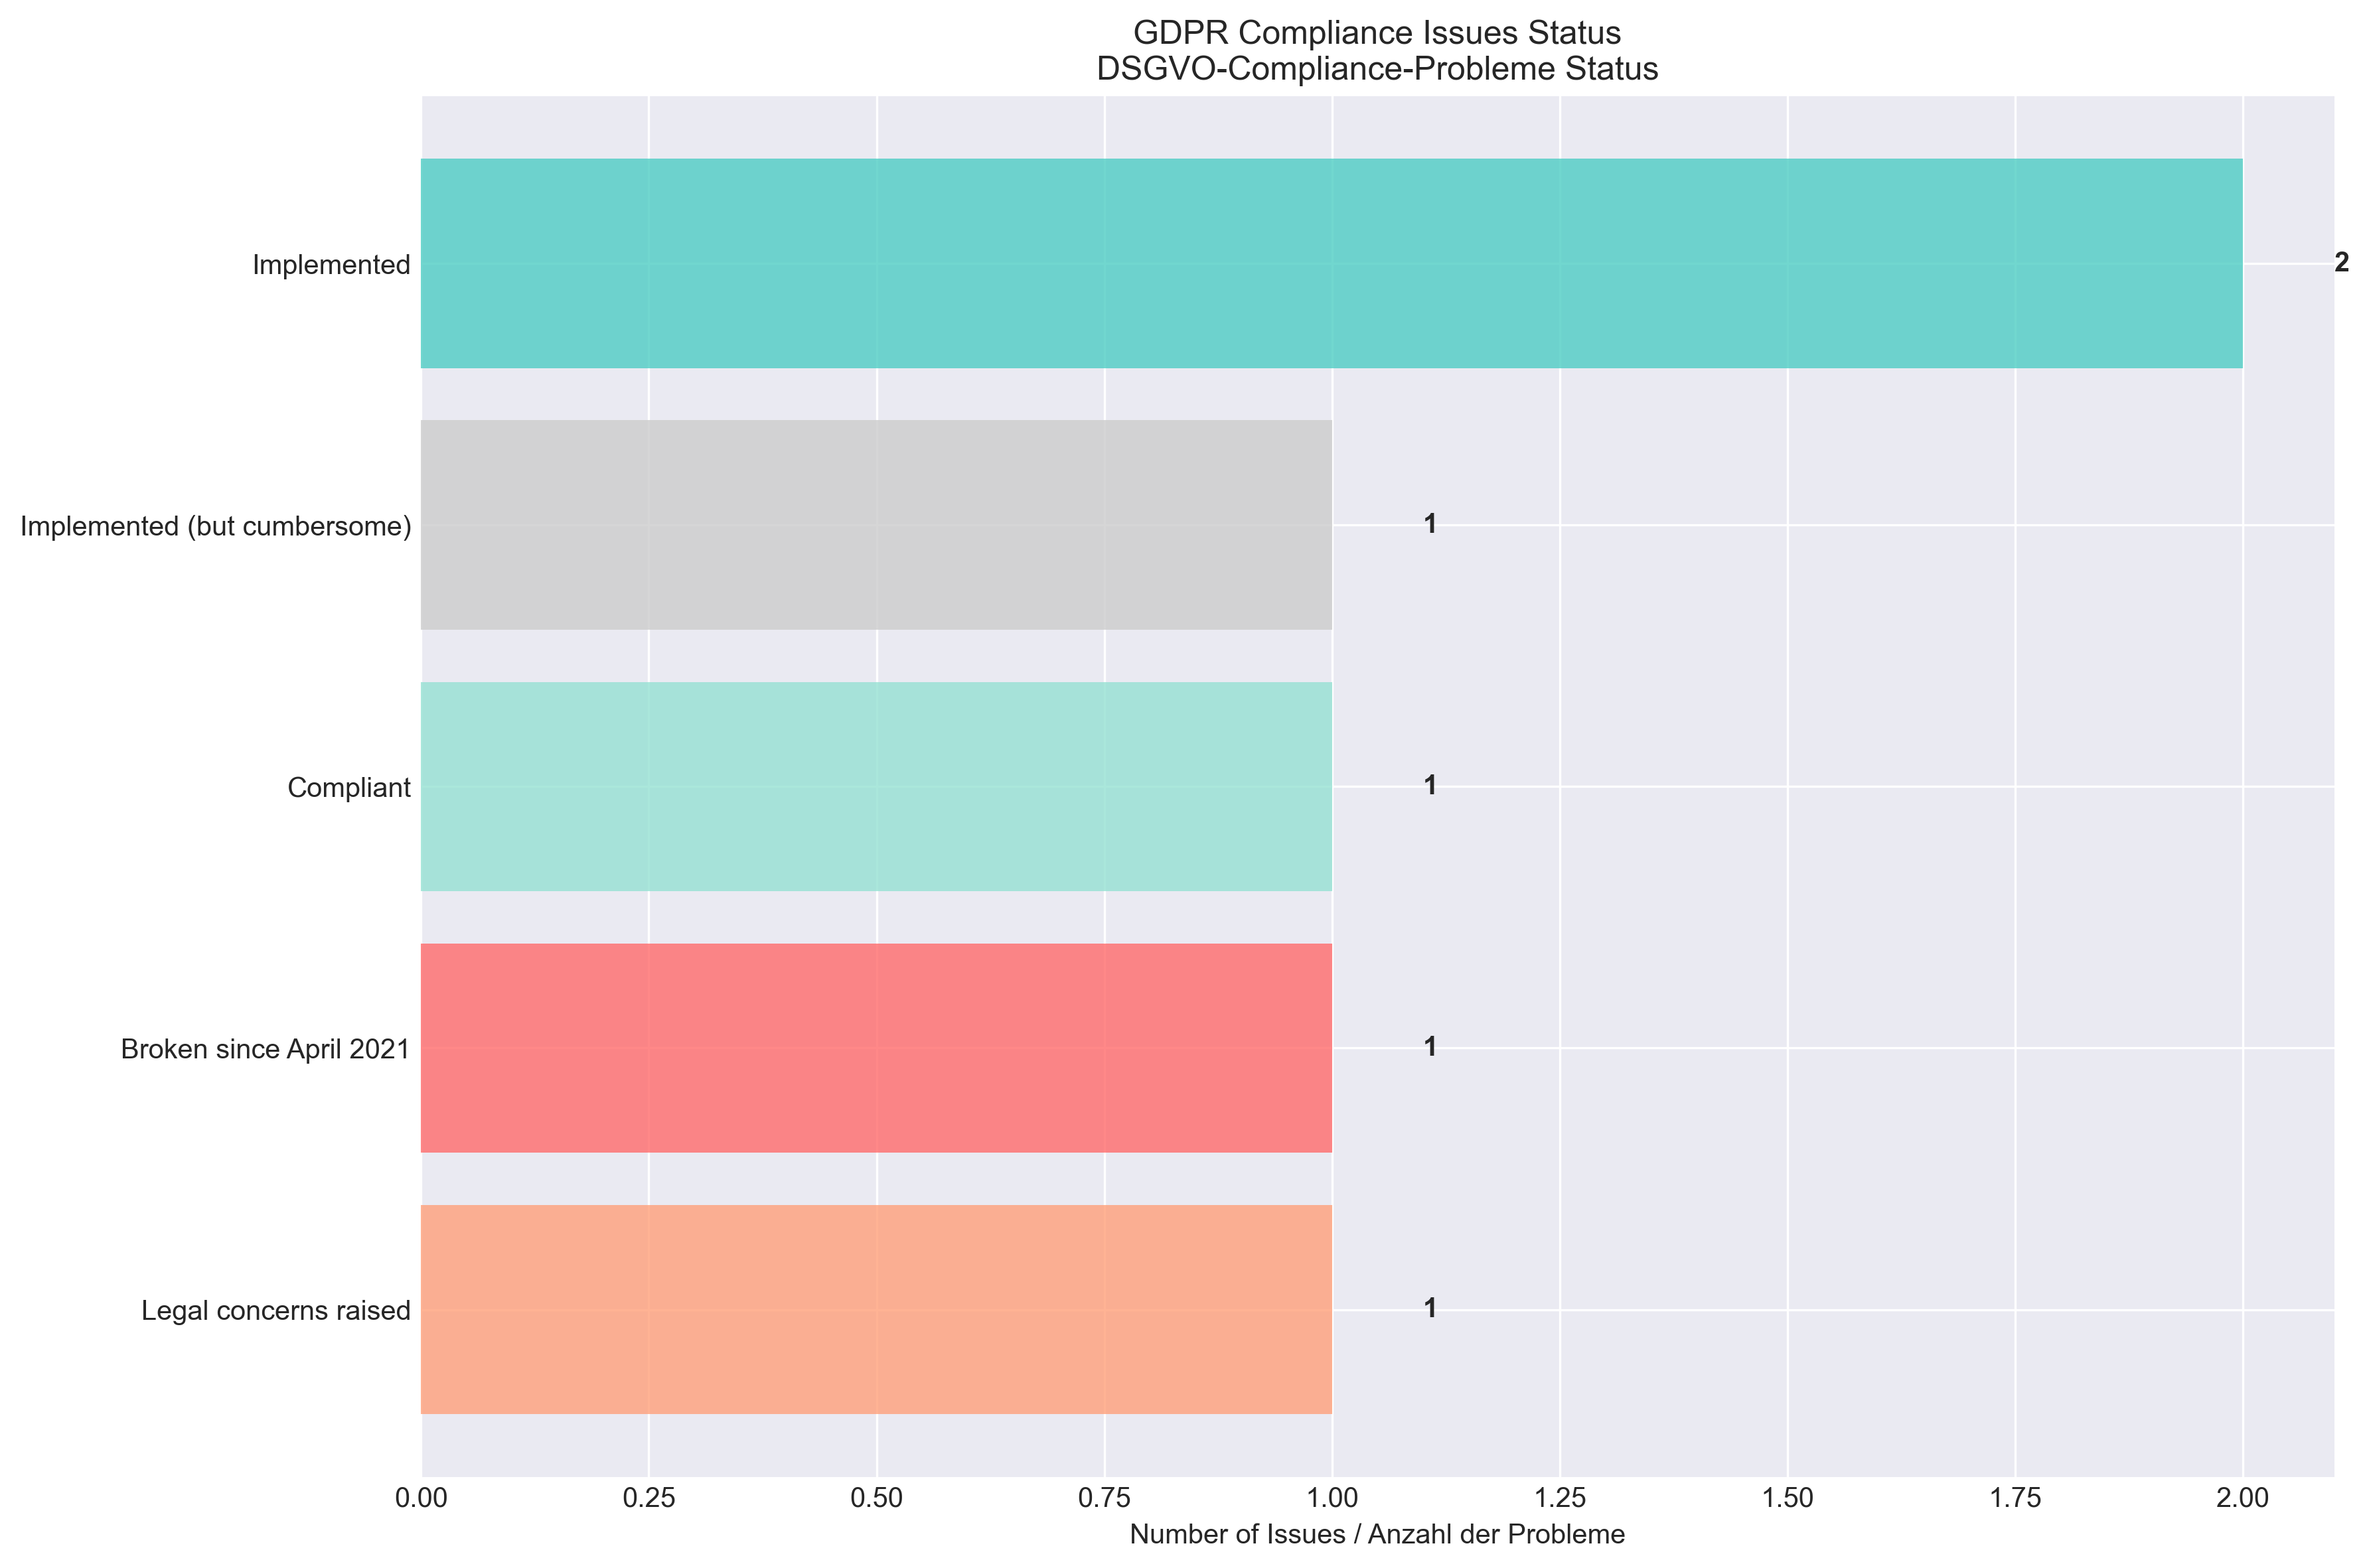
\includegraphics[width=0.9\textwidth]{figures/gdpr_compliance_status.png}
\caption{GDPR Compliance Issues Status / DSGVO-Compliance-Probleme Status}
\label{fig:gdpr-compliance}
\end{figure}

如图~\ref{fig:gdpr-compliance}所示，GDPR合规问题涉及多个方面，包括数据处理授权、数据存储位置、数据导出功能等。这些问题严重限制了WeChat在欧洲的运营模式。

As shown in Figure~\ref{fig:gdpr-compliance}, GDPR compliance issues involve multiple aspects, including data processing authorization, data storage location, data export functionality, etc. These issues severely restrict WeChat's operational model in Europe.

Wie in Abbildung~\ref{fig:gdpr-compliance} dargestellt, umfassen DSGVO-Compliance-Probleme mehrere Aspekte, einschließlich Datenverarbeitungsautorisierung, Datenspeicherort, Datenexportfunktionalität usw. Diese Probleme schränken WeChats Betriebsmodell in Europa erheblich ein.

\begin{itemize}
    \item \textbf{GDPR（通用数据保护条例）}：欧盟的GDPR对数据收集、处理和跨服务共享施加了严格限制。微信生态模式依赖于跨服务的数据整合和用户行为追踪，这在GDPR框架下面临重大合规挑战。
    \item \textbf{GDPR (General Data Protection Regulation)}: The EU's GDPR imposes strict limitations on data collection, processing, and cross-service sharing. WeChat's ecosystem model relies on cross-service data integration and user behavior tracking, which faces significant compliance challenges under the GDPR framework.
    \item \textbf{DSGVO (Datenschutz-Grundverordnung)}: Die DSGVO der EU setzt strenge Grenzen für Datensammlung, -verarbeitung und -austausch zwischen Diensten. WeChats Ökosystemmodell basiert auf dienstübergreifender Datenintegration und Nutzerverhaltensverfolgung, was erhebliche Compliance-Herausforderungen unter dem DSGVO-Rahmen darstellt.
    
    \item \textbf{数据最小化原则}：欧洲监管强调数据最小化，要求只收集必要的数据。微信的"一站式"服务模式需要收集大量用户数据以提供个性化服务，这与欧洲的隐私保护理念存在根本冲突。
    \item \textbf{Data Minimization Principle}: European regulations emphasize data minimization, requiring collection of only necessary data. WeChat's "all-in-one" service model requires collecting extensive user data to provide personalized services, fundamentally conflicting with Europe's privacy protection philosophy.
    \item \textbf{Datenminimierungsprinzip}: Europäische Vorschriften betonen die Datenminimierung und erfordern die Sammlung nur notwendiger Daten. WeChats "All-in-One"-Service-Modell erfordert die Sammlung umfangreicher Nutzerdaten für personalisierte Dienste, was grundlegend mit Europas Datenschutzphilosophie kollidiert.
    
    \item \textbf{用户同意要求}：GDPR要求明确的、具体的用户同意，禁止"一揽子"同意。微信生态需要用户同意多个服务的条款，这在GDPR下变得复杂。
    \item \textbf{User Consent Requirements}: GDPR requires explicit, specific user consent and prohibits "blanket" consent. WeChat's ecosystem requires user consent for multiple services' terms, which becomes complex under GDPR.
    \item \textbf{Nutzereinwilligungsanforderungen}: Die DSGVO erfordert ausdrückliche, spezifische Nutzereinwilligung und verbietet "Pauschal"-Einwilligung. WeChats Ökosystem erfordert Nutzereinwilligung für mehrere Dienstbedingungen, was unter der DSGVO komplex wird.
\end{itemize}

\subsection{反垄断监管 / Antitrust Regulations / Kartellrechtliche Vorschriften}

\textbf{欧盟的竞争政策 / EU Competition Policy / EU-Wettbewerbspolitik}

\begin{itemize}
    \item \textbf{市场支配地位限制}：欧盟对大型科技平台的垄断行为有严格监管。微信生态模式通过整合多个服务领域建立市场支配地位，这在欧盟反垄断框架下可能被视为滥用市场支配地位。
    \item \textbf{Market Dominance Restrictions}: The EU has strict regulations on monopolistic behavior by large tech platforms. WeChat's ecosystem model establishes market dominance by integrating multiple service areas, which may be considered abuse of market dominance under EU antitrust framework.
    \item \textbf{Marktbeherrschungsbeschränkungen}: Die EU hat strenge Vorschriften für monopolistisches Verhalten großer Technologieplattformen. WeChats Ökosystemmodell etabliert Marktbeherrschung durch Integration mehrerer Dienstbereiche, was als Missbrauch der Marktbeherrschung unter dem EU-Kartellrecht angesehen werden könnte.
    
    \item \textbf{"二选一"等排他性行为}：微信生态中的排他性策略（如要求商家在微信和其他平台之间选择）在欧盟可能违反竞争法。欧盟对这类行为有明确的禁止规定。
    \item \textbf{Exclusive Practices like "Pick One"}: Exclusive strategies in WeChat's ecosystem (such as requiring merchants to choose between WeChat and other platforms) may violate competition law in the EU. The EU has clear prohibitions on such practices.
    \item \textbf{Exklusive Praktiken wie "Wähle eins"}: Exklusive Strategien in WeChats Ökosystem (wie die Anforderung, dass Händler zwischen WeChat und anderen Plattformen wählen) könnten gegen das Wettbewerbsrecht in der EU verstoßen. Die EU hat klare Verbote für solche Praktiken.
    
    \item \textbf{数字市场法案（DMA）}：欧盟的DMA对"守门人"平台施加了额外义务，限制其整合服务的能力，进一步阻碍了超级应用模式。
    \item \textbf{Digital Markets Act (DMA)}: The EU's DMA imposes additional obligations on "gatekeeper" platforms, limiting their ability to integrate services, further hindering the super-app model.
    \item \textbf{Digital Markets Act (DMA)}: Der DMA der EU setzt zusätzliche Verpflichtungen für "Torwächter"-Plattformen fest und schränkt ihre Fähigkeit zur Dienstintegration ein, was das Super-App-Modell weiter behindert.
\end{itemize}

\subsection{金融服务监管 / Financial Services Regulation / Finanzdienstleistungsregulierung}

\textbf{支付服务指令（PSD2）等法规 / Payment Services Directive (PSD2) and Other Regulations / Zahlungsdiensterichtlinie (PSD2) und andere Vorschriften}

\begin{itemize}
    \item \textbf{开放银行要求}：欧盟的PSD2要求银行向第三方支付服务提供商开放API，促进支付市场的竞争。这与微信支付在中国相对封闭的生态形成对比。
    \item \textbf{Open Banking Requirements}: The EU's PSD2 requires banks to open APIs to third-party payment service providers, promoting competition in the payment market. This contrasts with WeChat Pay's relatively closed ecosystem in China.
    \item \textbf{Open-Banking-Anforderungen}: Die PSD2 der EU verlangt, dass Banken APIs für Drittanbieter-Zahlungsdienstleister öffnen, um Wettbewerb im Zahlungsmarkt zu fördern. Dies steht im Gegensatz zu WeChat Pays relativ geschlossenem Ökosystem in China.
    
    \item \textbf{金融牌照要求}：在欧洲提供支付服务需要获得相应的金融牌照，监管门槛较高。微信支付作为中国产品，在欧洲获得金融牌照面临更多障碍。
    \item \textbf{Financial License Requirements}: Providing payment services in Europe requires obtaining appropriate financial licenses, with high regulatory barriers. WeChat Pay, as a Chinese product, faces additional obstacles in obtaining financial licenses in Europe.
    \item \textbf{Finanzlizenzanforderungen}: Die Bereitstellung von Zahlungsdiensten in Europa erfordert entsprechende Finanzlizenzen mit hohen regulatorischen Barrieren. WeChat Pay als chinesisches Produkt steht vor zusätzlichen Hindernissen bei der Erlangung von Finanzlizenzen in Europa.
    
    \item \textbf{反洗钱（AML）要求}：欧洲对支付服务提供商有严格的反洗钱合规要求，需要建立复杂的合规体系。
    \item \textbf{Anti-Money Laundering (AML) Requirements}: Europe has strict AML compliance requirements for payment service providers, requiring establishment of complex compliance systems.
    \item \textbf{Anti-Geldwäsche (AML)-Anforderungen}: Europa hat strenge AML-Compliance-Anforderungen für Zahlungsdienstleister, die die Einrichtung komplexer Compliance-Systeme erfordern.
\end{itemize}

\section{市场结构与竞争格局 / Market Structure and Competitive Landscape / Marktstruktur und Wettbewerbslandschaft}

\subsection{市场碎片化 / Market Fragmentation / Marktfragmentierung}

\textbf{欧洲多国市场的复杂性 / Complexity of Multi-Country European Markets / Komplexität der mehrstaatlichen europäischen Märkte}

\begin{itemize}
    \item \textbf{27+个独立市场}：欧盟由27个成员国组成，每个国家有自己的语言、文化、法规和消费者习惯。微信需要为每个市场进行本地化，成本极高。
    \item \textbf{27+ Independent Markets}: The EU consists of 27 member states, each with its own language, culture, regulations, and consumer habits. WeChat would need localization for each market, with extremely high costs.
    \item \textbf{27+ unabhängige Märkte}: Die EU besteht aus 27 Mitgliedstaaten, jeder mit eigener Sprache, Kultur, Vorschriften und Verbrauchergewohnheiten. WeChat müsste für jeden Markt lokalisiert werden, mit extrem hohen Kosten.
    
    \item \textbf{语言障碍}：欧洲有24种官方语言，微信需要支持多语言界面和内容，这增加了开发和运营的复杂性。
    \item \textbf{Language Barriers}: Europe has 24 official languages. WeChat would need to support multilingual interfaces and content, increasing development and operational complexity.
    \item \textbf{Sprachbarrieren}: Europa hat 24 Amtssprachen. WeChat müsste mehrsprachige Schnittstellen und Inhalte unterstützen, was die Entwicklungs- und Betriebskomplexität erhöht.
\end{itemize}

\begin{figure}[ht]
\centering
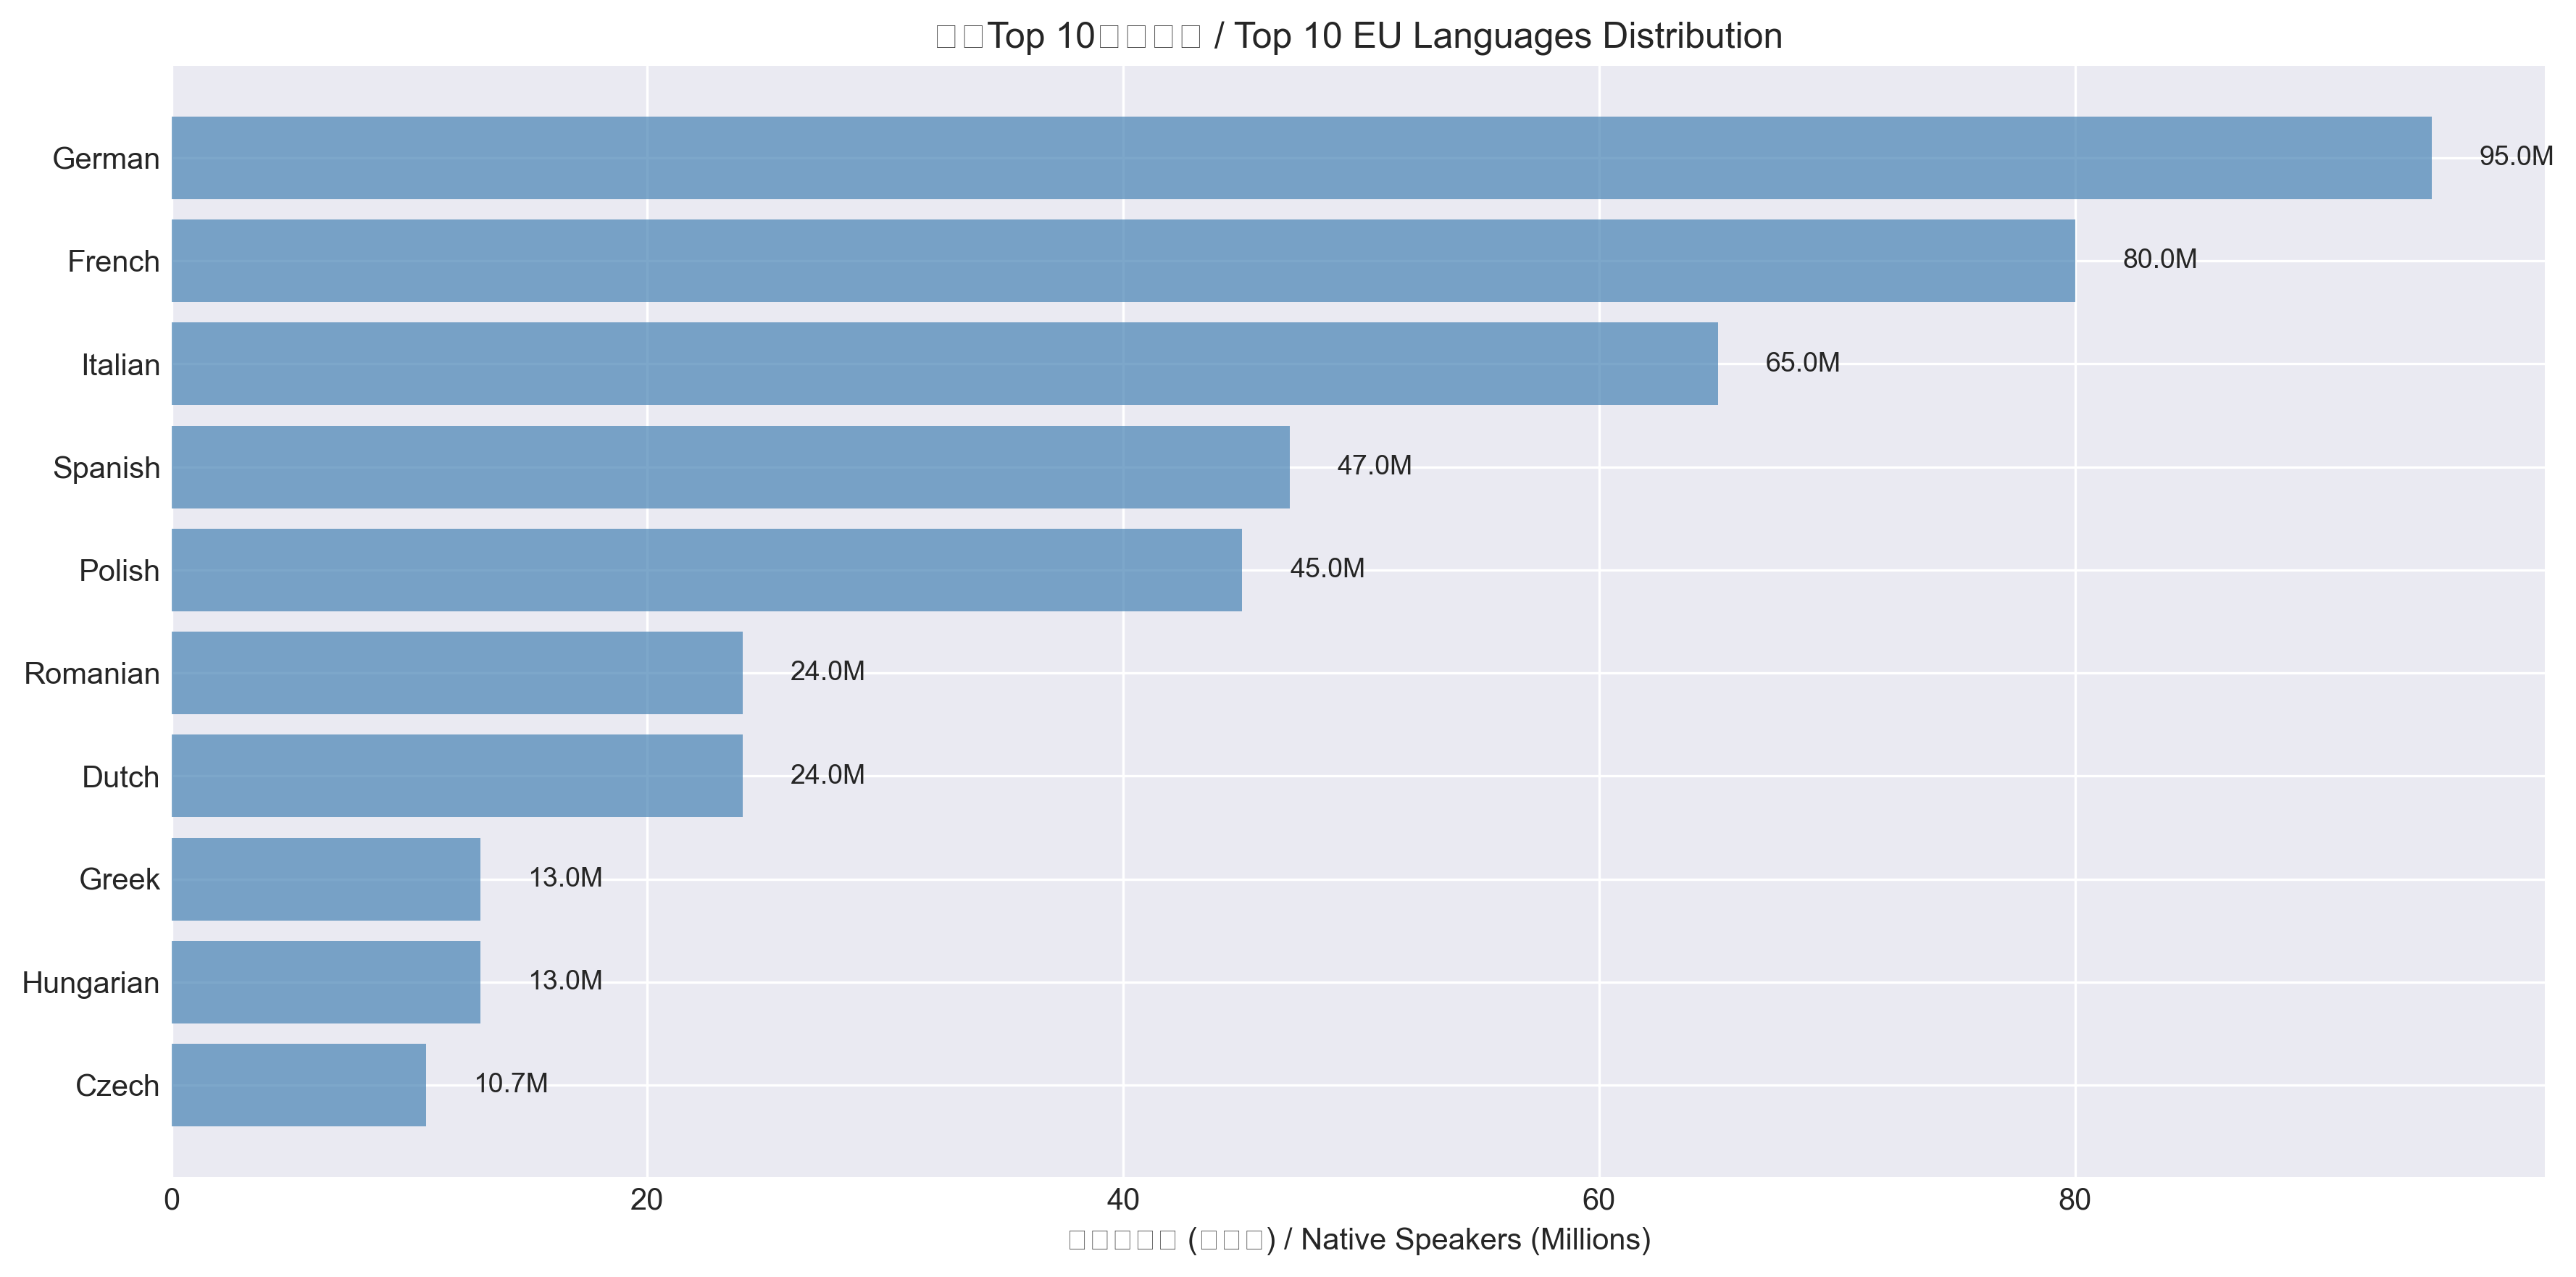
\includegraphics[width=0.9\textwidth]{figures/eu_languages.png}
\caption{Top 10 EU Languages Distribution / Top 10 EU-Sprachen-Verteilung}
\label{fig:eu-languages}
\end{figure}

如图~\ref{fig:eu-languages}所示，欧盟有24种官方语言，其中德语、法语、意大利语、西班牙语等主要语言的使用者数量庞大，这要求WeChat进行大量的本地化工作。

As shown in Figure~\ref{fig:eu-languages}, the EU has 24 official languages, with major languages such as German, French, Italian, and Spanish having large numbers of speakers, requiring extensive localization work from WeChat.

Wie in Abbildung~\ref{fig:eu-languages} dargestellt, hat die EU 24 Amtssprachen, wobei Hauptsprachen wie Deutsch, Französisch, Italienisch und Spanisch eine große Anzahl von Sprechern haben, was umfangreiche Lokalisierungsarbeiten von WeChat erfordert.

\begin{itemize}
    
    \item \textbf{法规差异}：每个成员国可能有不同的数据保护、支付、电商法规，需要分别合规。
    \item \textbf{Regulatory Differences}: Each member state may have different data protection, payment, and e-commerce regulations, requiring separate compliance.
    \item \textbf{Regulatorische Unterschiede}: Jeder Mitgliedstaat kann unterschiedliche Datenschutz-, Zahlungs- und E-Commerce-Vorschriften haben, was separate Compliance erfordert.
\end{itemize}

\subsection{既有竞争者的市场地位 / Established Competitors' Market Position / Marktposition etablierter Wettbewerber}

\textbf{已占据各细分市场的成熟平台 / Mature Platforms Already Dominating Market Segments / Reife Plattformen, die bereits Marktsegmente dominieren}

\begin{itemize}
    \item \textbf{通讯领域}：WhatsApp和Telegram已经占据欧洲即时通讯市场的主导地位，用户迁移成本高。根据2024年数据，WhatsApp在欧洲有超过4亿用户。
    \item \textbf{Messaging Sector}: WhatsApp and Telegram already dominate the European instant messaging market, with high user switching costs. According to 2024 data, WhatsApp has over 400 million users in Europe.
    \item \textbf{Messaging-Bereich}: WhatsApp und Telegram dominieren bereits den europäischen Instant-Messaging-Markt mit hohen Nutzerwechselkosten. Laut Daten von 2024 hat WhatsApp über 400 Millionen Nutzer in Europa.
\end{itemize}

\begin{figure}[ht]
\centering
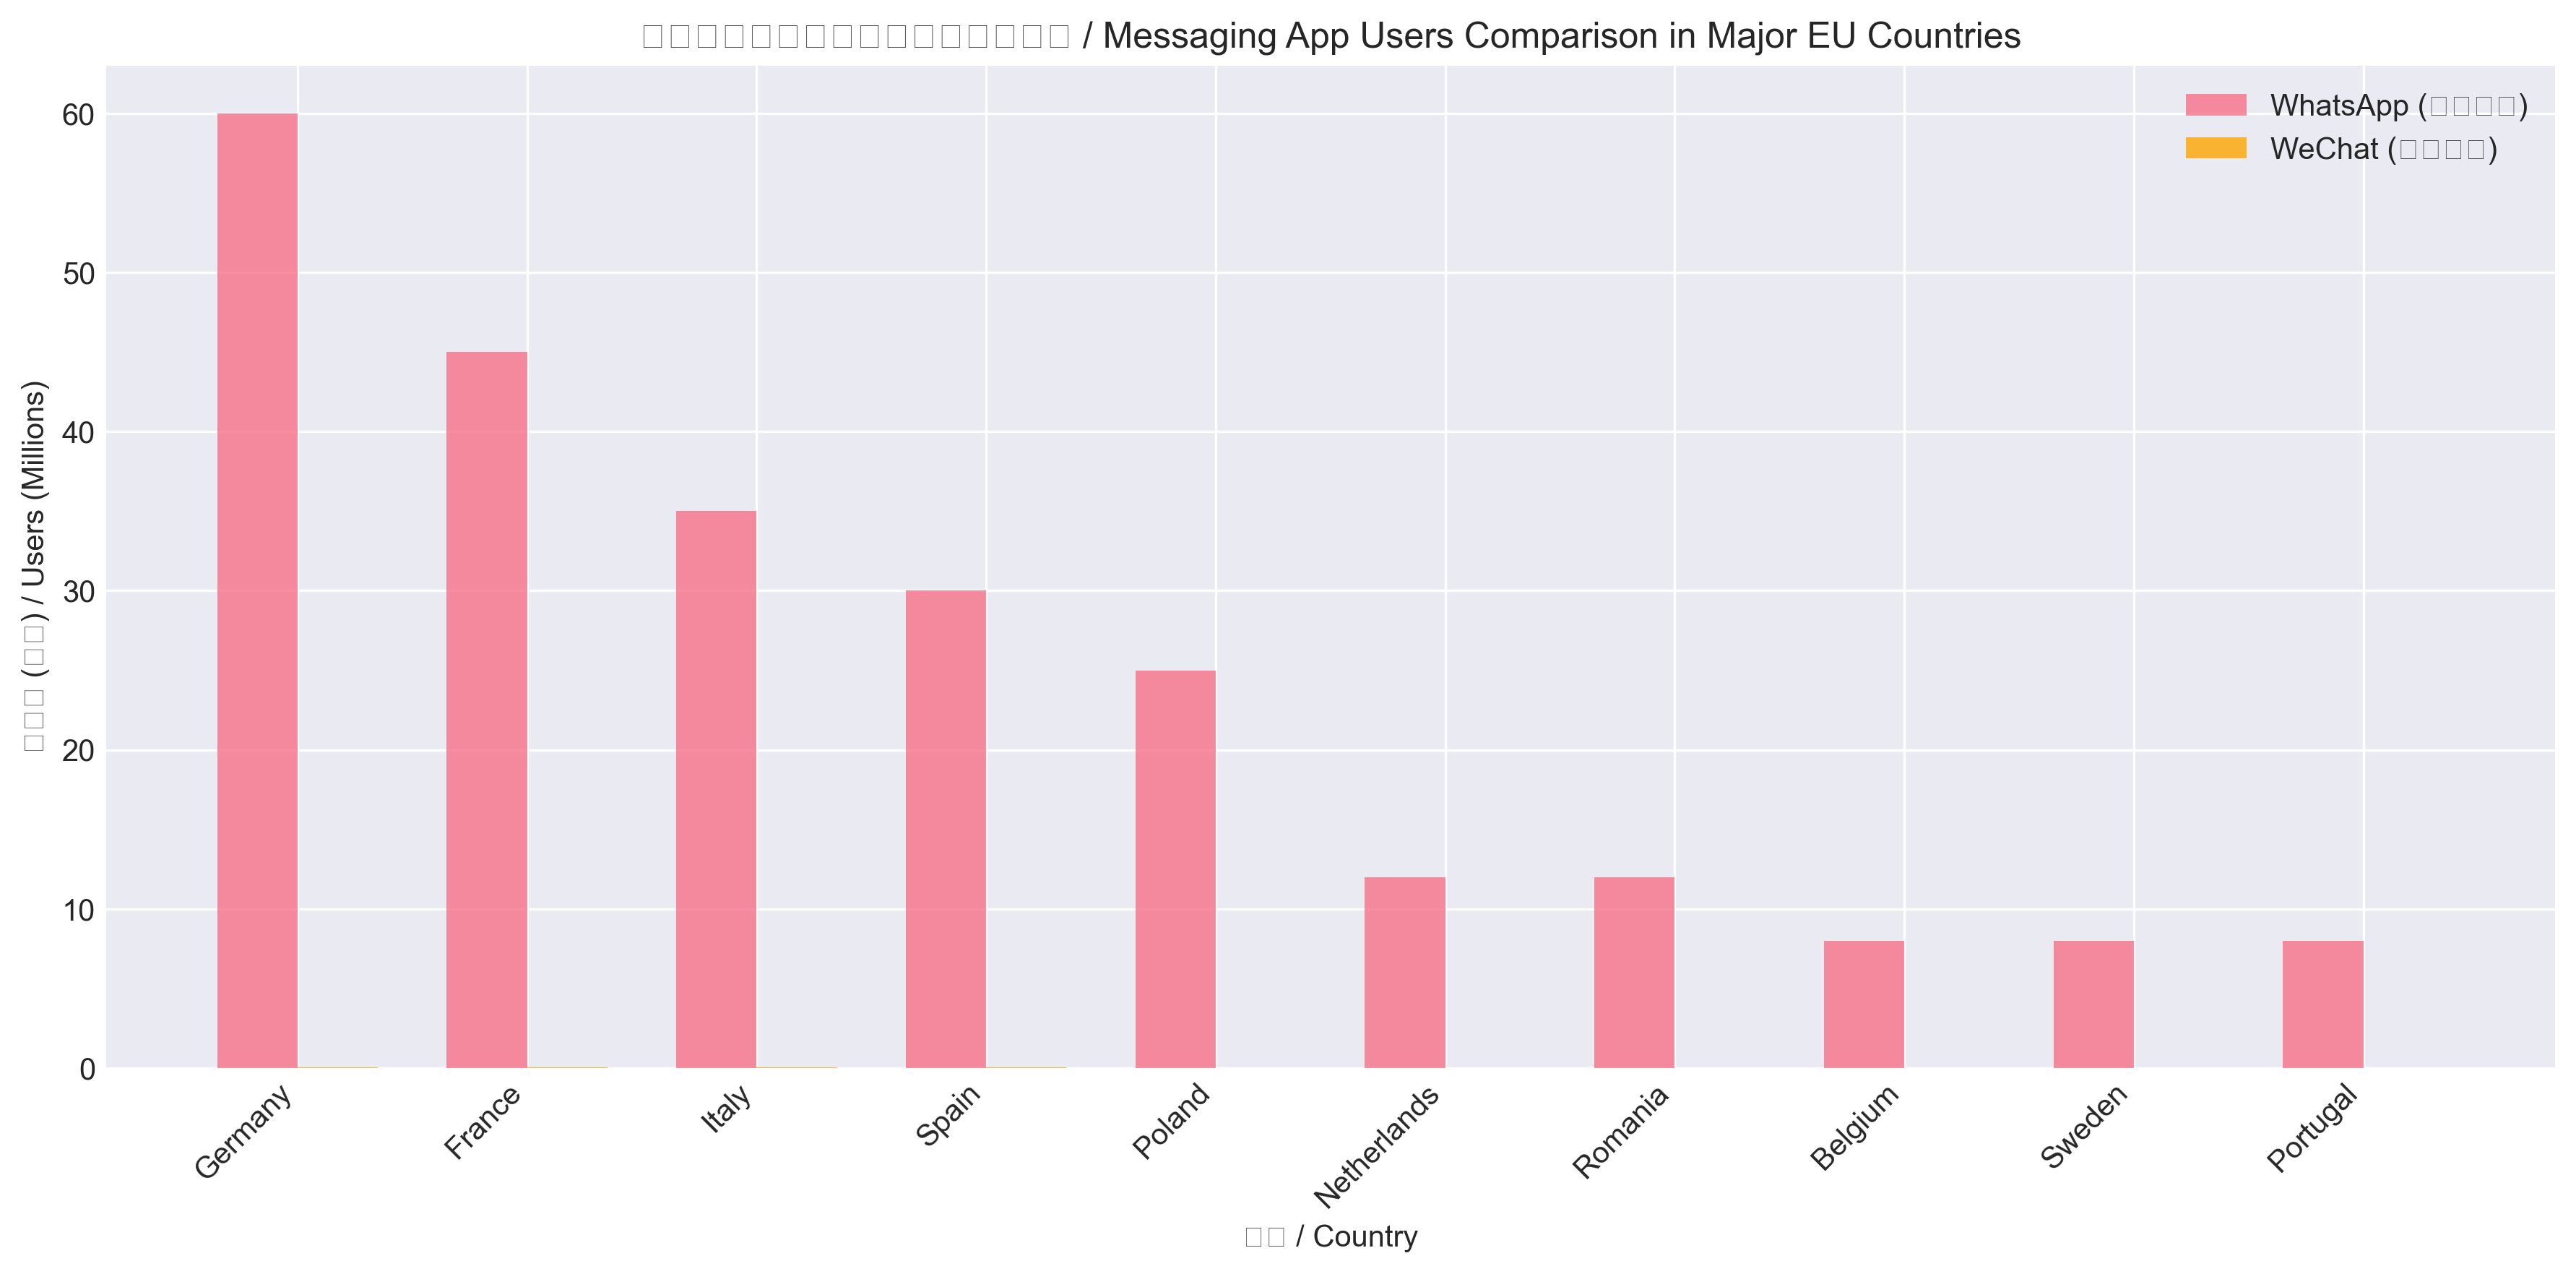
\includegraphics[width=0.9\textwidth]{figures/messaging_app_comparison.png}
\caption{Messaging App Users Comparison in Major EU Countries / Messaging-App-Nutzervergleich in wichtigen EU-Ländern}
\label{fig:messaging-comparison}
\end{figure}

\begin{figure}[ht]
\centering
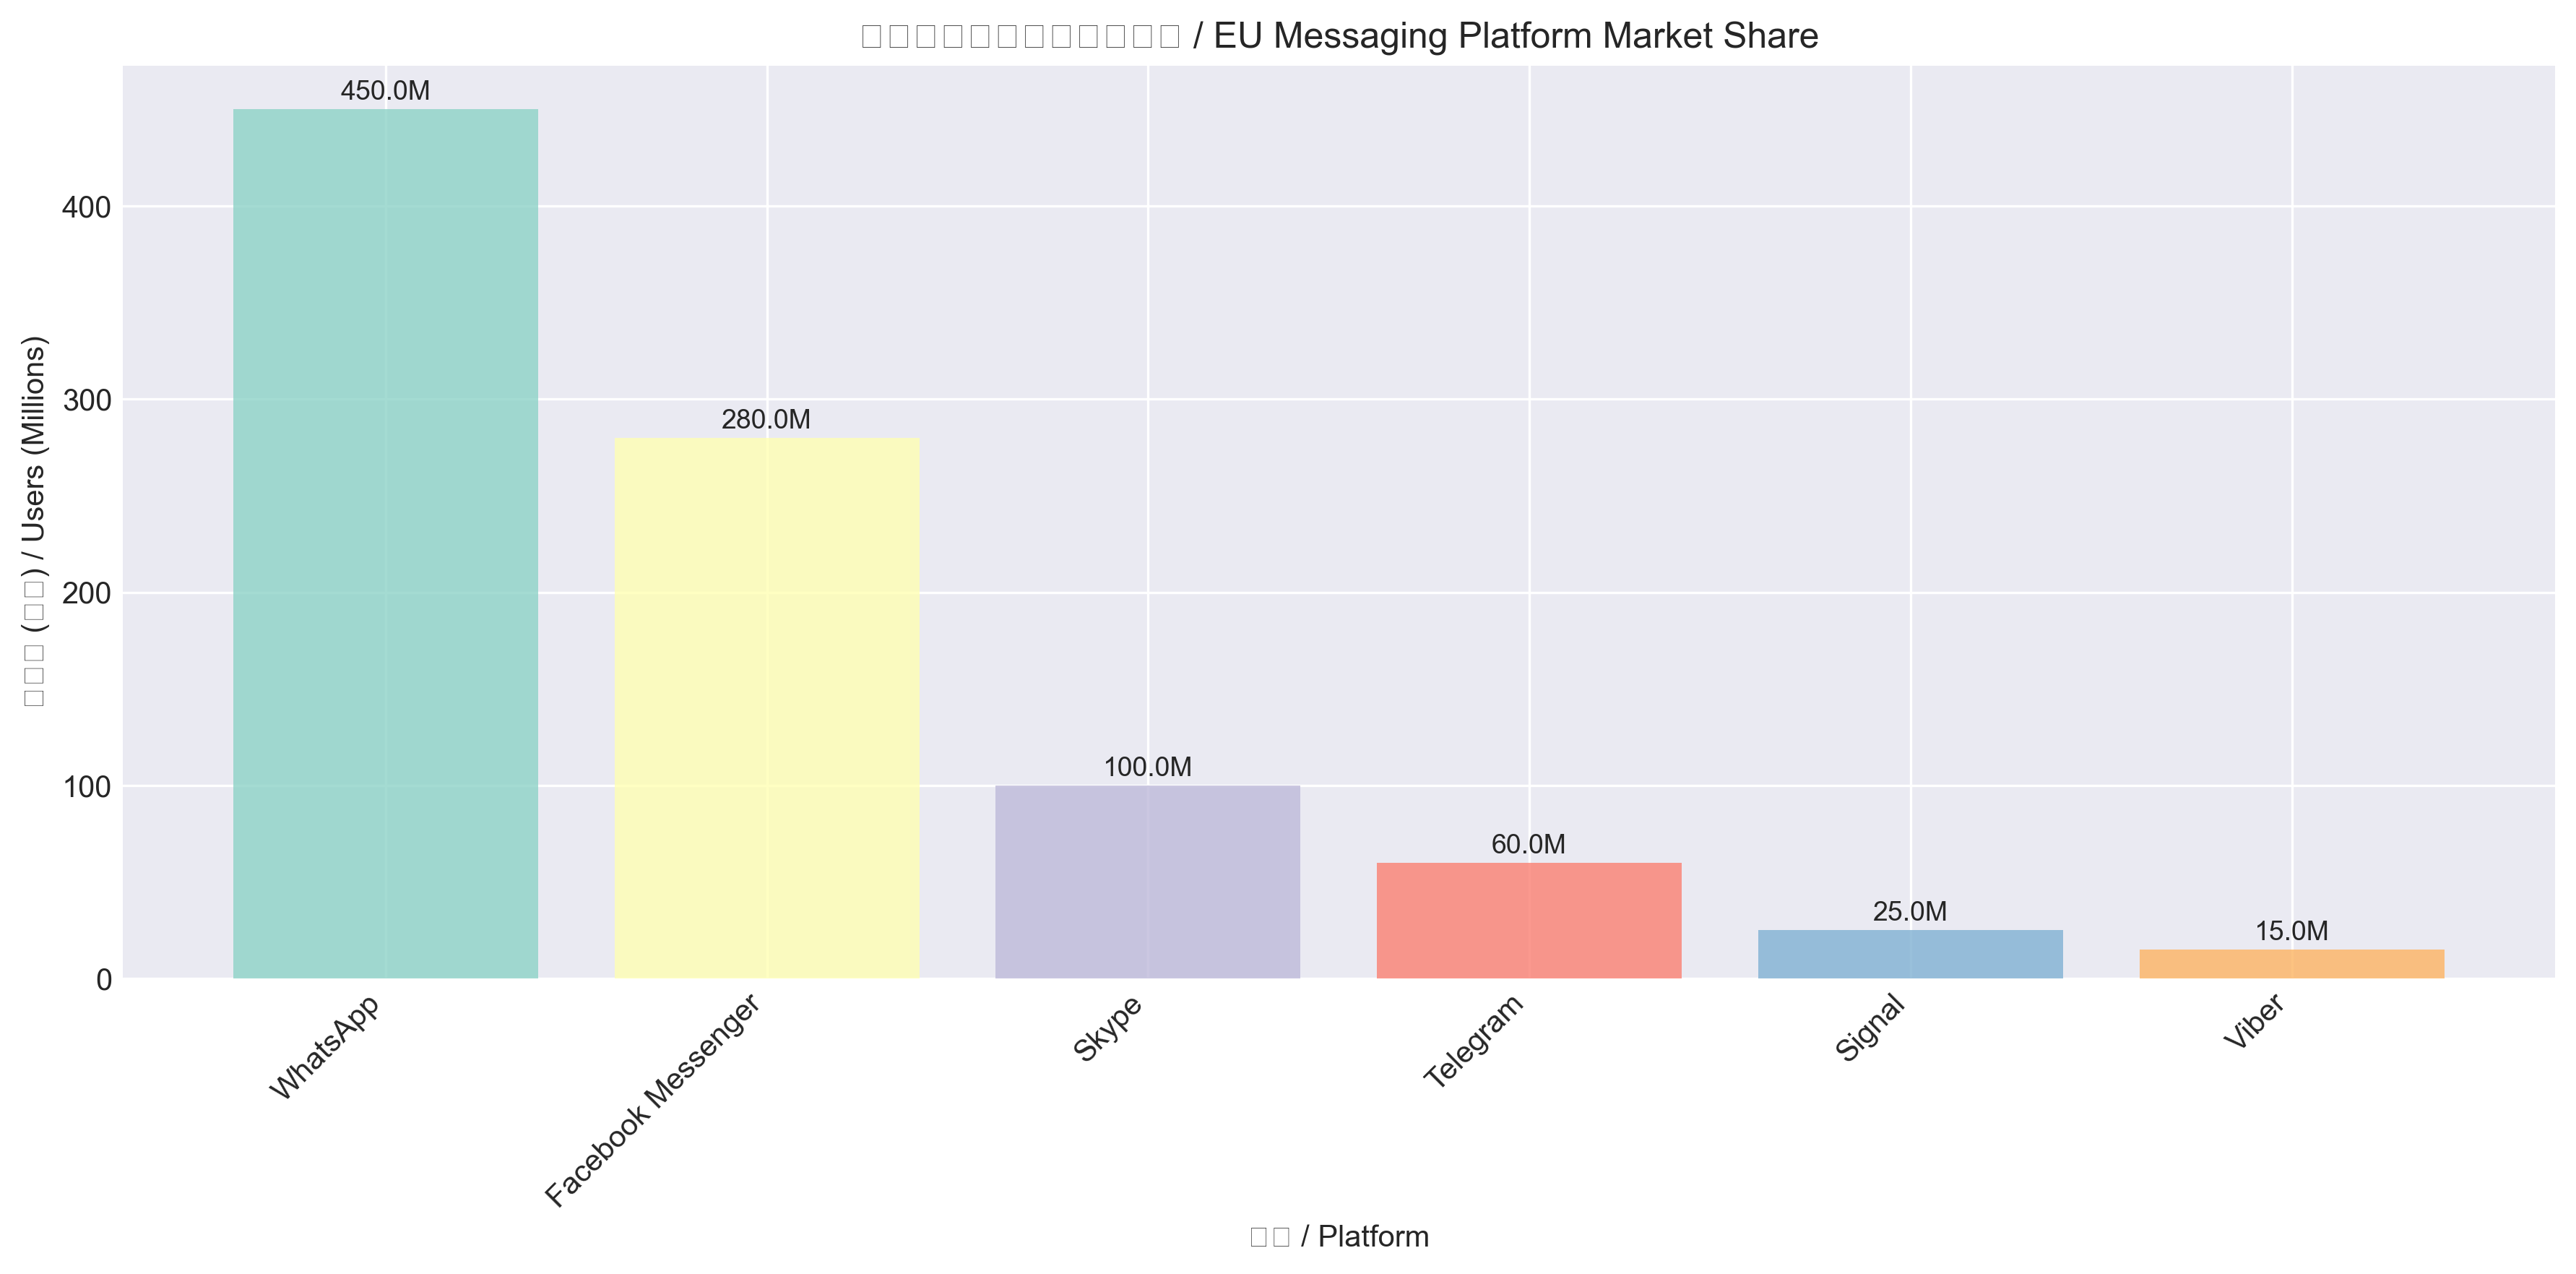
\includegraphics[width=0.9\textwidth]{figures/platform_market_share.png}
\caption{EU Messaging Platform Market Share / EU-Messaging-Plattform-Marktanteil}
\label{fig:platform-share}
\end{figure}

如图~\ref{fig:messaging-comparison}和图~\ref{fig:platform-share}所示，WhatsApp在欧洲主要国家占据绝对主导地位，而WeChat的用户数几乎可以忽略不计。这反映了欧洲即时通讯市场的成熟度和竞争格局。

As shown in Figures~\ref{fig:messaging-comparison} and~\ref{fig:platform-share}, WhatsApp dominates absolutely in major European countries, while WeChat's user numbers are almost negligible. This reflects the maturity and competitive landscape of the European instant messaging market.

Wie in den Abbildungen~\ref{fig:messaging-comparison} und~\ref{fig:platform-share} dargestellt, dominiert WhatsApp absolut in wichtigen europäischen Ländern, während WeChats Nutzerzahlen fast vernachlässigbar sind. Dies spiegelt die Reife und Wettbewerbslandschaft des europäischen Instant-Messaging-Markts wider.

\begin{itemize}
    
    \item \textbf{支付领域}：PayPal、Stripe、Apple Pay、Google Pay等已建立强大的市场地位，用户习惯已形成。欧洲移动支付市场已被这些平台分割。
    \item \textbf{Payment Sector}: PayPal, Stripe, Apple Pay, Google Pay have established strong market positions, with user habits already formed. The European mobile payment market is already divided among these platforms.
    \item \textbf{Zahlungsbereich}: PayPal, Stripe, Apple Pay, Google Pay haben starke Marktpositionen etabliert, Nutzergewohnheiten sind bereits gebildet. Der europäische mobile Zahlungsmarkt ist bereits unter diesen Plattformen aufgeteilt.
    
    \item \textbf{社交网络}：Facebook、Instagram、LinkedIn等已满足欧洲用户的社交需求，形成了强大的网络效应。
    \item \textbf{Social Networks}: Facebook, Instagram, LinkedIn already meet European users' social networking needs, forming strong network effects.
    \item \textbf{Soziale Netzwerke}: Facebook, Instagram, LinkedIn erfüllen bereits die sozialen Netzwerkbedürfnisse europäischer Nutzer und bilden starke Netzwerkeffekte.
    
    \item \textbf{电商平台}：Amazon、eBay等电商平台在欧洲已有强大地位，微信难以在电商领域建立竞争优势。
    \item \textbf{E-Commerce Platforms}: Amazon, eBay and other e-commerce platforms already have strong positions in Europe, making it difficult for WeChat to establish competitive advantages in e-commerce.
    \item \textbf{E-Commerce-Plattformen}: Amazon, eBay und andere E-Commerce-Plattformen haben bereits starke Positionen in Europa, was es WeChat schwer macht, Wettbewerbsvorteile im E-Commerce zu etablieren.
\end{itemize}

\subsection{网络效应的反向作用 / Reverse Network Effects / Umgekehrte Netzwerkeffekte}

\textbf{用户迁移的障碍 / Barriers to User Migration / Barrieren für Nutzermigration}

\begin{itemize}
    \item \textbf{现有网络锁定}：欧洲用户已经在现有平台上建立了社交网络和关系，迁移到新平台意味着失去这些连接。这是典型的网络锁定效应。
    \item \textbf{Existing Network Lock-in}: European users have already established social networks and relationships on existing platforms. Migrating to a new platform means losing these connections. This is a typical network lock-in effect.
    \item \textbf{Bestehende Netzwerksperre}: Europäische Nutzer haben bereits soziale Netzwerke und Beziehungen auf bestehenden Plattformen etabliert. Die Migration zu einer neuen Plattform bedeutet den Verlust dieser Verbindungen. Dies ist ein typischer Netzwerksperreffekt.
    
    \item \textbf{多平台使用习惯}：欧洲用户习惯于在不同平台上使用不同服务，而不是将所有活动集中在一个应用内。这种习惯难以改变。
    \item \textbf{Multi-Platform Usage Habits}: European users are accustomed to using different services on different platforms, rather than concentrating all activities within a single app. This habit is difficult to change.
    \item \textbf{Multi-Plattform-Nutzungsgewohnheiten}: Europäische Nutzer sind gewohnt, verschiedene Dienste auf verschiedenen Plattformen zu nutzen, anstatt alle Aktivitäten in einer App zu konzentrieren. Diese Gewohnheit ist schwer zu ändern.
    
    \item \textbf{数据迁移成本}：用户在不同平台间迁移数据（联系人、聊天记录、支付信息等）成本高，进一步阻碍了平台切换。
    \item \textbf{Data Migration Costs}: The cost of migrating data (contacts, chat history, payment information, etc.) between platforms is high, further hindering platform switching.
    \item \textbf{Datenmigrationskosten}: Die Kosten für die Migration von Daten (Kontakte, Chat-Verlauf, Zahlungsinformationen, etc.) zwischen Plattformen sind hoch und behindern Plattformwechsel weiter.
\end{itemize}

\section{用户行为与文化差异 / User Behavior and Cultural Differences / Nutzerverhalten und kulturelle Unterschiede}

\subsection{应用使用习惯 / Application Usage Habits / Anwendungsnutzungsgewohnheiten}

\textbf{专业化 vs 集成化偏好 / Specialization vs. Integration Preferences / Spezialisierung vs. Integrationspräferenzen}

\begin{figure}[ht]
\centering
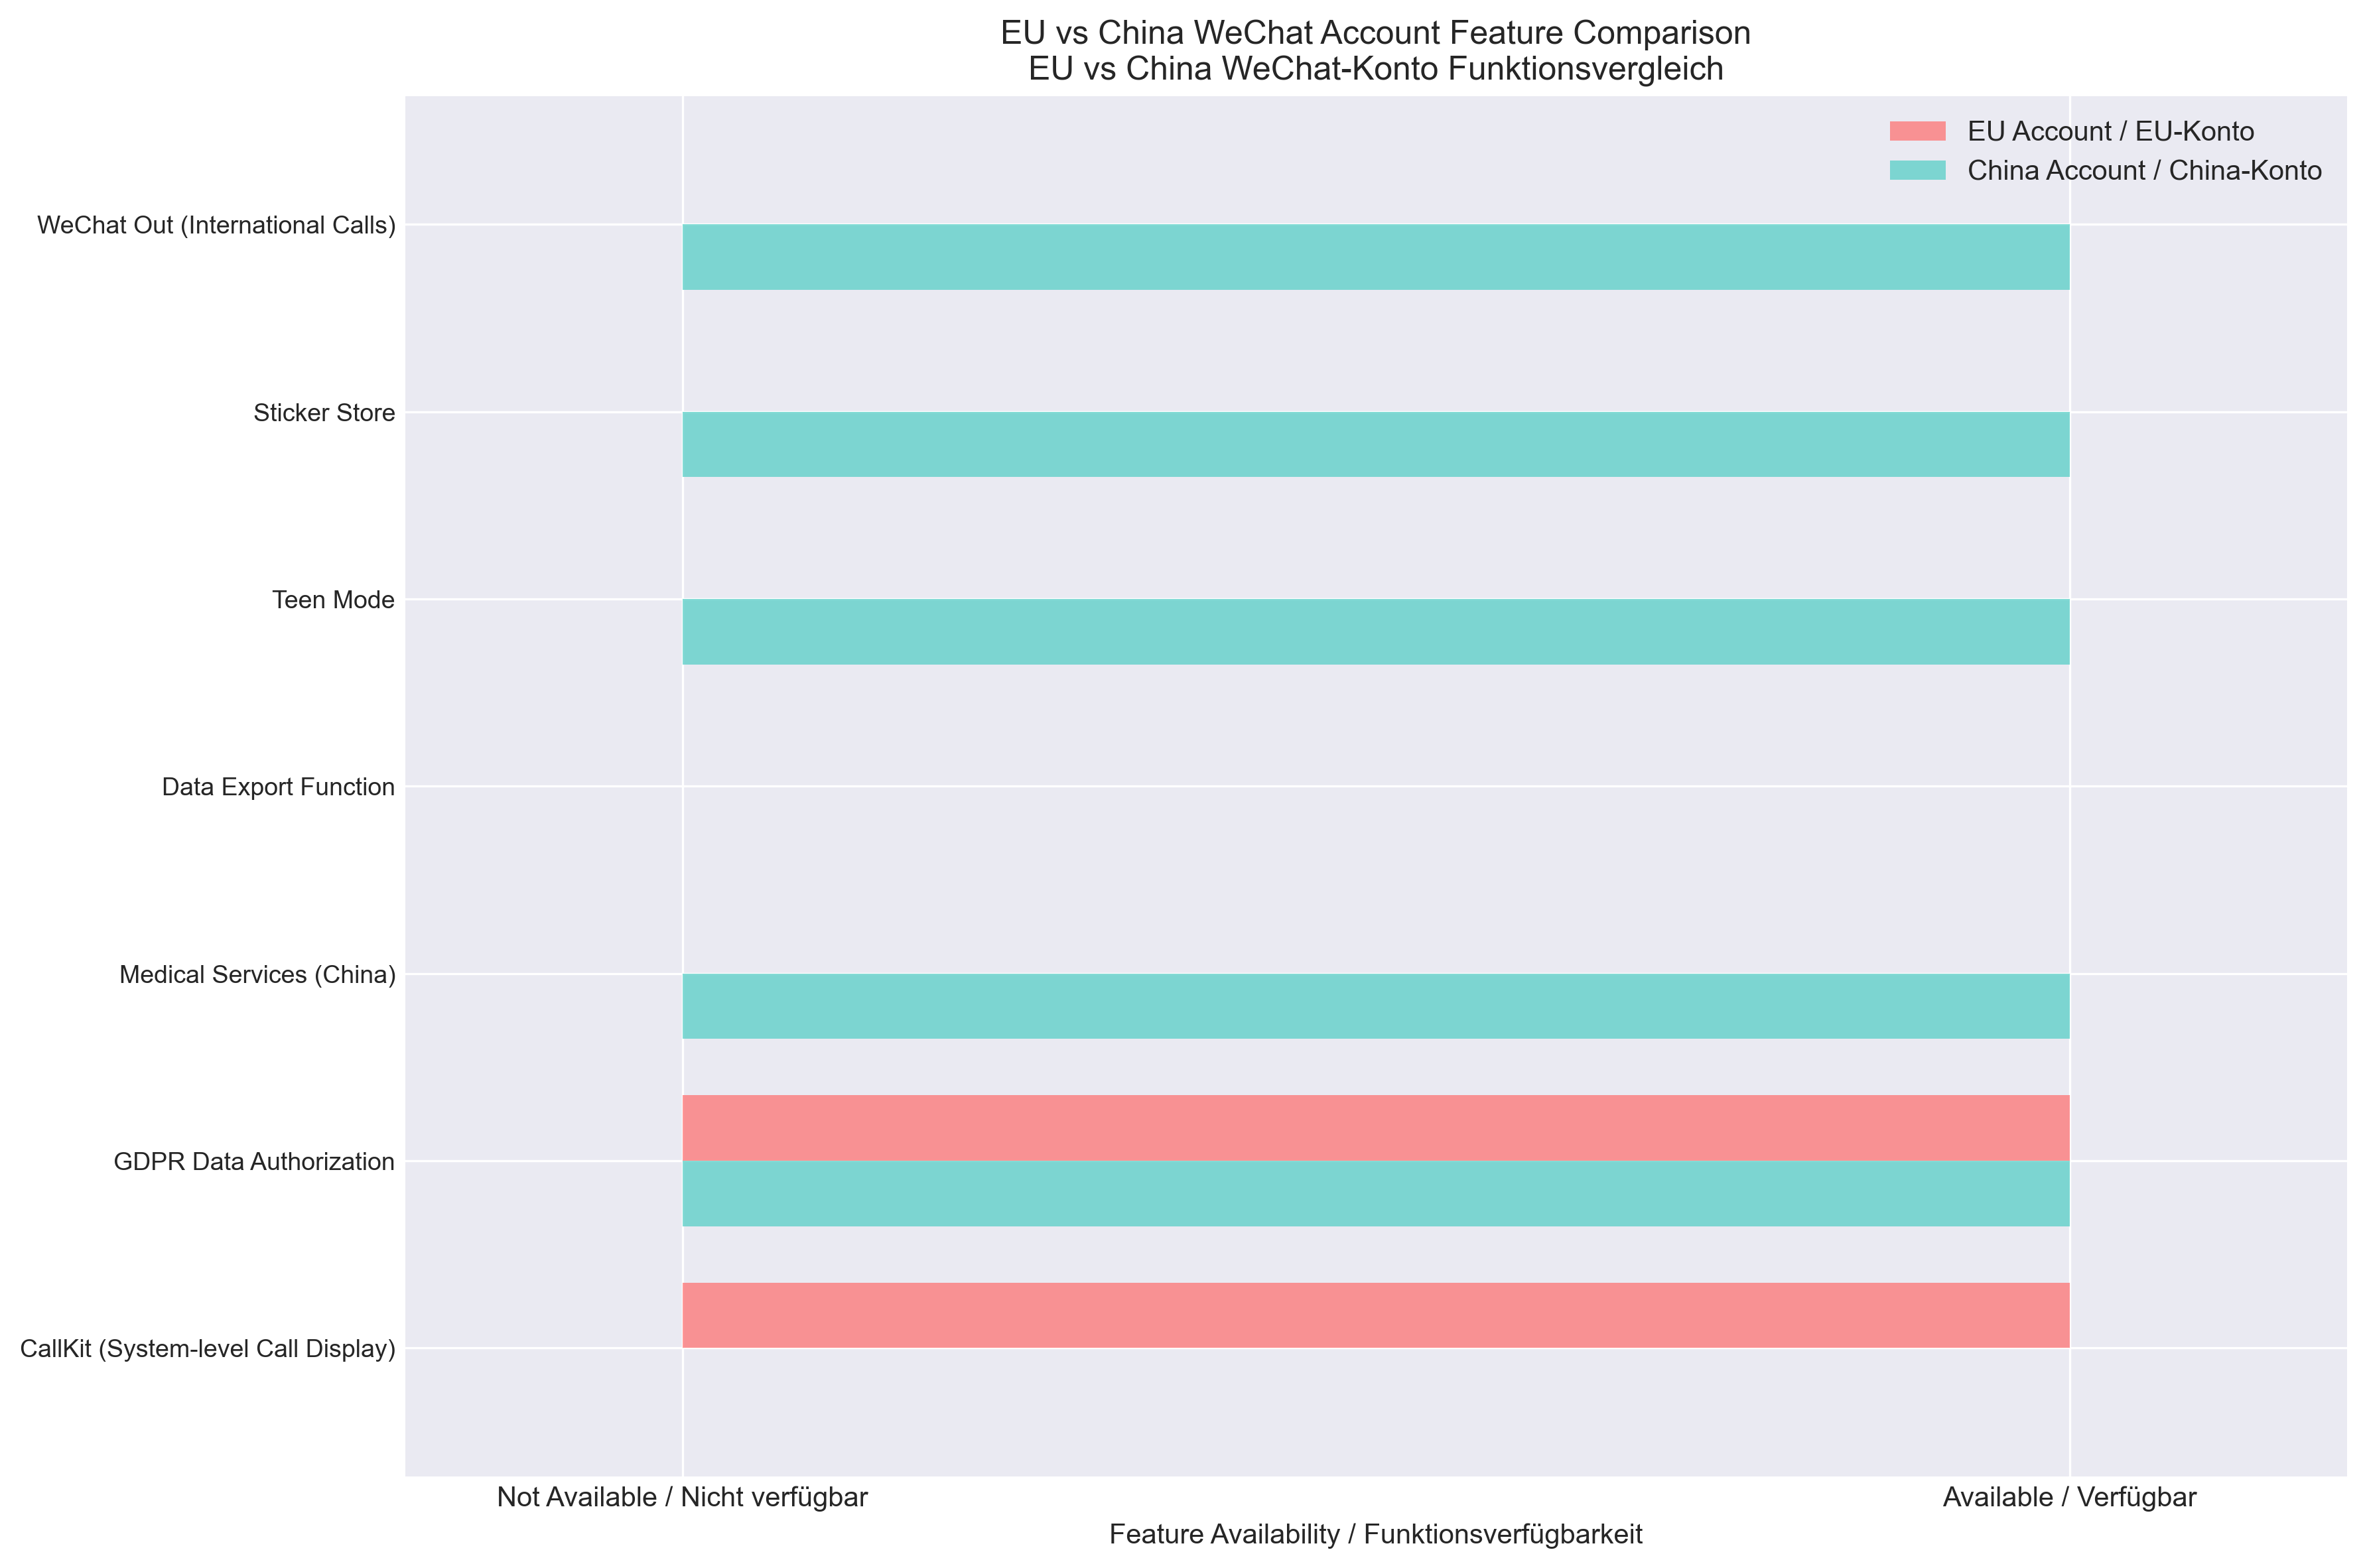
\includegraphics[width=0.9\textwidth]{figures/eu_china_wechat_comparison.png}
\caption{EU vs China WeChat Account Feature Comparison / EU vs China WeChat-Konto Funktionsvergleich}
\label{fig:eu-china-comparison}
\end{figure}

如图~\ref{fig:eu-china-comparison}所示，欧盟WeChat账户相比中国微信账户存在显著的功能限制。多个关键功能在欧盟账户中不可用或存在严重问题，这反映了GDPR监管要求和功能本地化的挑战。

As shown in Figure~\ref{fig:eu-china-comparison}, EU WeChat accounts have significant functional limitations compared to Chinese WeChat accounts. Multiple key features are unavailable or have serious issues in EU accounts, reflecting GDPR regulatory requirements and functional localization challenges.

Wie in Abbildung~\ref{fig:eu-china-comparison} dargestellt, haben EU-WeChat-Konten erhebliche funktionale Einschränkungen im Vergleich zu chinesischen WeChat-Konten. Mehrere Schlüsselfunktionen sind in EU-Konten nicht verfügbar oder haben schwerwiegende Probleme, was die DSGVO-Regulierungsanforderungen und funktionale Lokalisierungsherausforderungen widerspiegelt.

\begin{itemize}
    \item \textbf{功能分离偏好}：欧洲用户更倾向于使用专门化的应用，每个应用专注于特定功能。他们认为这样更安全、更可控、更符合"单一职责原则"。
    \item \textbf{Preference for Functional Separation}: European users prefer specialized applications, with each app focusing on specific functions. They consider this safer, more controllable, and more aligned with the "single responsibility principle."
    \item \textbf{Präferenz für funktionale Trennung}: Europäische Nutzer bevorzugen spezialisierte Anwendungen, wobei jede App auf spezifische Funktionen fokussiert. Sie betrachten dies als sicherer, kontrollierbarer und besser mit dem "Single-Responsibility-Prinzip" übereinstimmend.
    
    \item \textbf{隐私意识}：欧洲用户对数据隐私有更强的意识，不愿意将所有个人信息和活动集中在一个平台上。他们担心数据集中带来的隐私风险。
    \item \textbf{Privacy Awareness}: European users have stronger awareness of data privacy and are unwilling to concentrate all personal information and activities on a single platform. They worry about privacy risks from data concentration.
    \item \textbf{Datenschutzbewusstsein}: Europäische Nutzer haben ein stärkeres Bewusstsein für Datenschutz und sind nicht bereit, alle persönlichen Informationen und Aktivitäten auf einer einzigen Plattform zu konzentrieren. Sie sorgen sich um Datenschutzrisiken durch Datenkonzentration.
    
    \item \textbf{应用商店文化}：欧洲用户习惯于从应用商店下载独立应用，每个应用有明确的功能定位，这与微信的"应用内应用"模式不同。
    \item \textbf{App Store Culture}: European users are accustomed to downloading independent apps from app stores, with each app having clear functional positioning, which differs from WeChat's "app-within-app" model.
    \item \textbf{App-Store-Kultur}: Europäische Nutzer sind gewohnt, unabhängige Apps aus App-Stores herunterzuladen, wobei jede App eine klare funktionale Positionierung hat, was sich von WeChats "App-in-App"-Modell unterscheidet.
\end{itemize}

\subsection{支付习惯差异 / Payment Habit Differences / Unterschiede in Zahlungsgewohnheiten}

\textbf{成熟的支付基础设施 / Mature Payment Infrastructure / Reife Zahlungsinfrastruktur}

\begin{itemize}
    \item \textbf{银行卡普及率高}：欧洲银行卡（信用卡、借记卡）普及率极高，用户已经习惯使用银行卡支付，对移动支付的依赖度较低。根据欧洲央行数据，2023年欧洲银行卡支付占非现金支付的70\%以上。
    \item \textbf{High Bank Card Penetration}: Europe has extremely high bank card (credit, debit) penetration. Users are already accustomed to card payments and have lower dependence on mobile payments. According to European Central Bank data, card payments accounted for over 70\% of non-cash payments in Europe in 2023.
    \item \textbf{Hohe Bankkarten-Durchdringung}: Europa hat eine extrem hohe Bankkarten-Durchdringung (Kredit-, Debitkarten). Nutzer sind bereits an Kartenzahlungen gewöhnt und haben geringere Abhängigkeit von mobilen Zahlungen. Laut Daten der Europäischen Zentralbank machten Kartenzahlungen 2023 über 70\% der bargeldlosen Zahlungen in Europa aus.
\end{itemize}

\begin{figure}[ht]
\centering
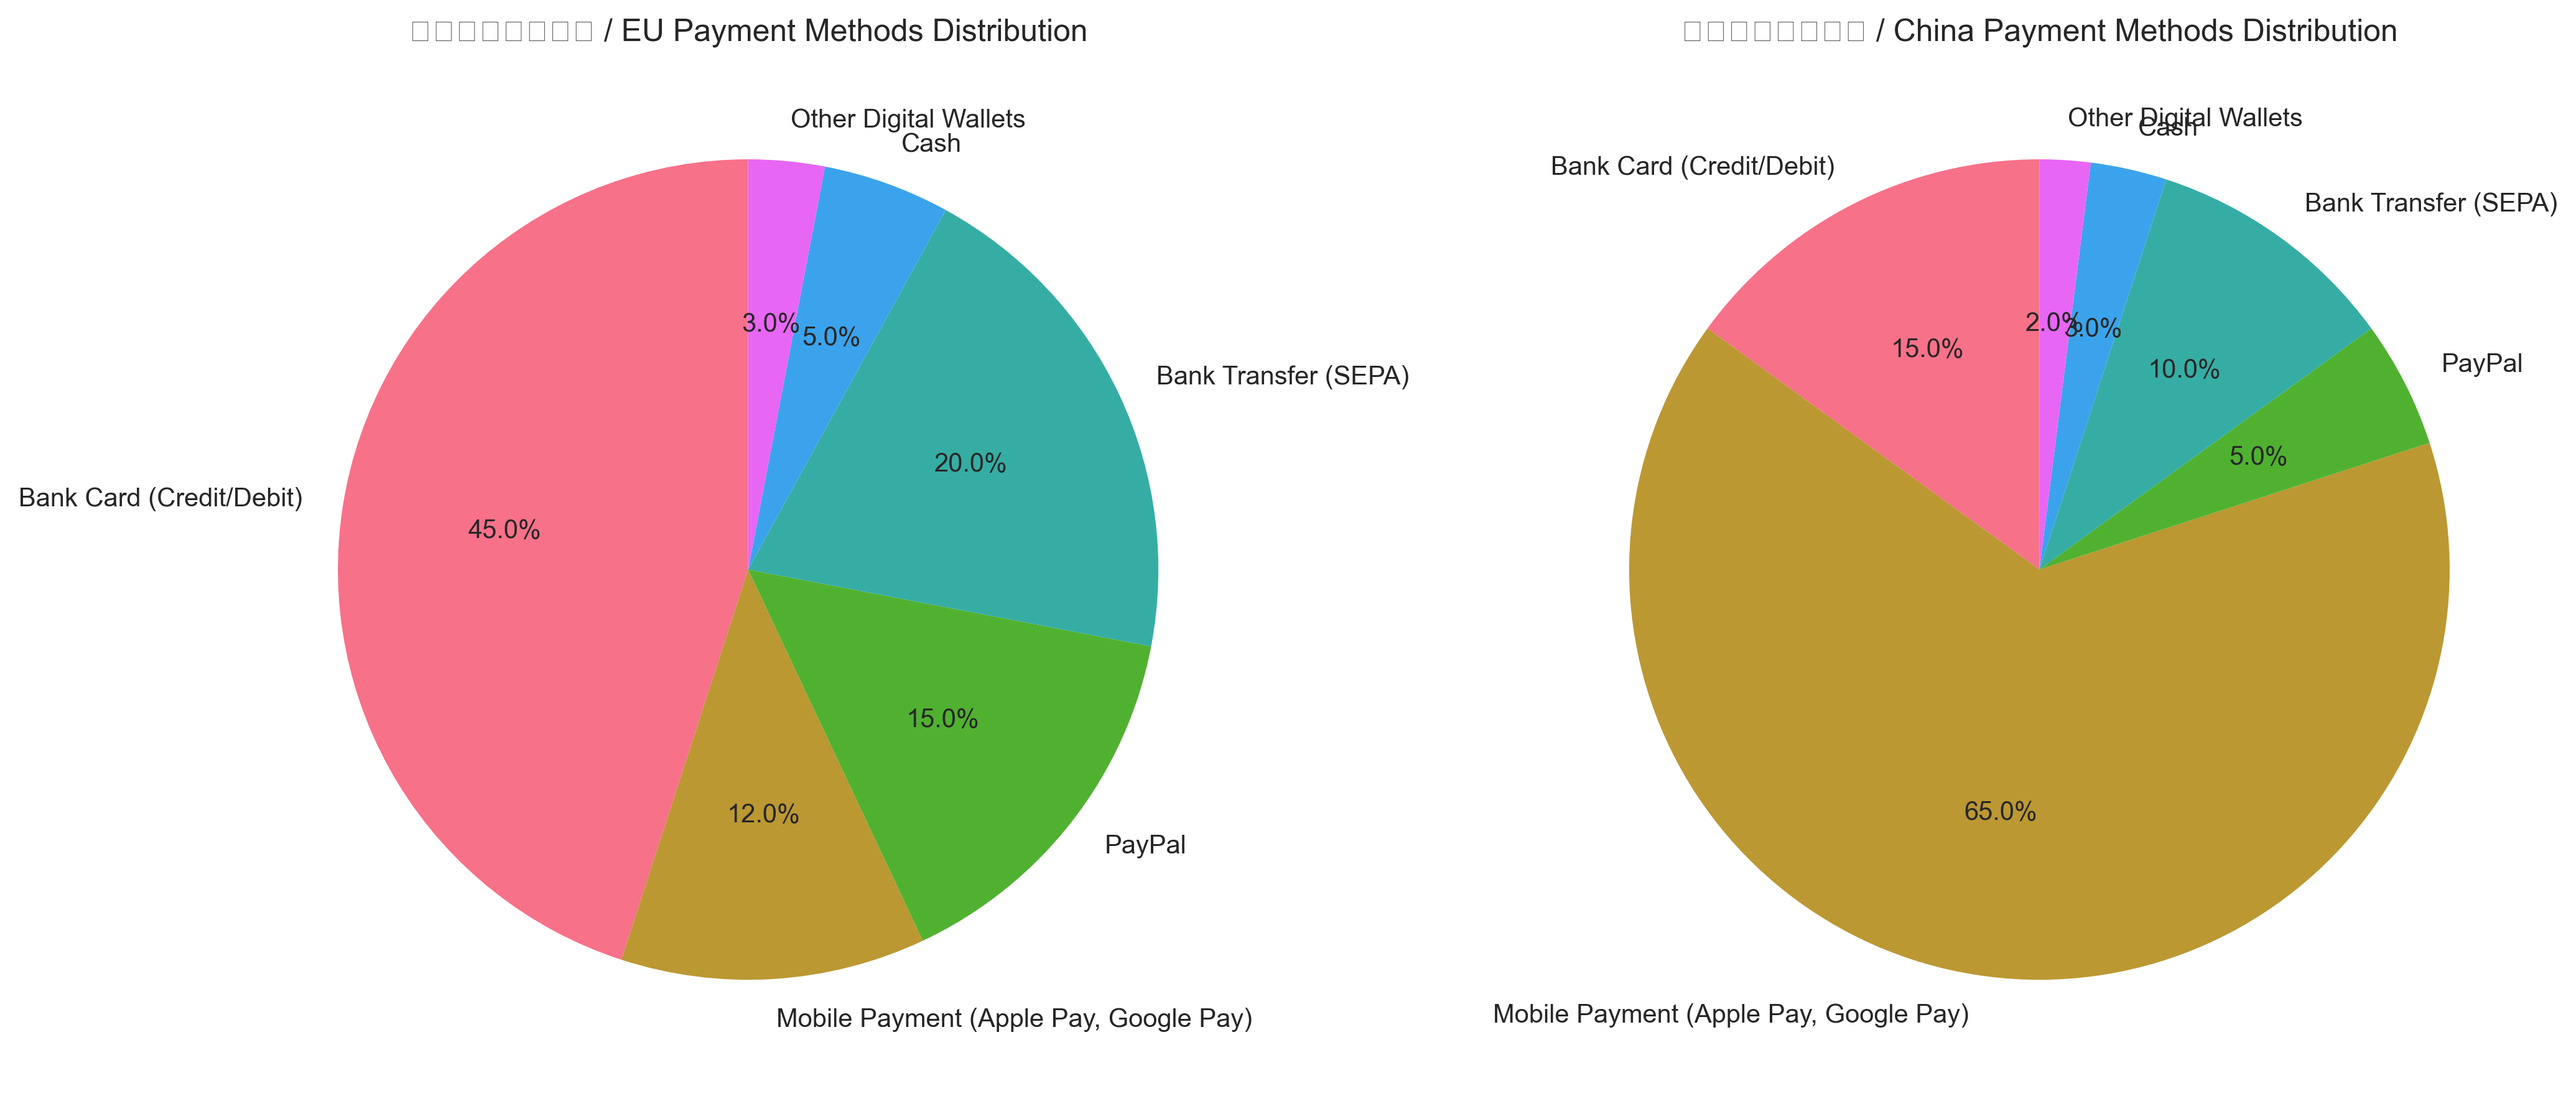
\includegraphics[width=0.9\textwidth]{figures/payment_methods_comparison.png}
\caption{EU vs China Payment Methods Distribution / EU vs China Zahlungsmethoden-Verteilung}
\label{fig:payment-methods}
\end{figure}

如图~\ref{fig:payment-methods}所示，欧洲和中国在支付方式上存在根本性差异。欧洲依赖银行卡和传统支付方式，而中国以移动支付为主导。这种差异反映了两个市场在支付基础设施和用户习惯上的不同。

As shown in Figure~\ref{fig:payment-methods}, there are fundamental differences in payment methods between Europe and China. Europe relies on bank cards and traditional payment methods, while China is dominated by mobile payments. This difference reflects the different payment infrastructure and user habits in the two markets.

Wie in Abbildung~\ref{fig:payment-methods} dargestellt, gibt es grundlegende Unterschiede in den Zahlungsmethoden zwischen Europa und China. Europa verlässt sich auf Bankkarten und traditionelle Zahlungsmethoden, während China von mobilen Zahlungen dominiert wird. Dieser Unterschied spiegelt die unterschiedliche Zahlungsinfrastruktur und Nutzergewohnheiten in den beiden Märkten wider.

\begin{itemize}
    
    \item \textbf{多种支付方式并存}：欧洲市场已有多种成熟的支付解决方案（SEPA转账、PayPal、Apple Pay、Google Pay、各种本地支付方式），用户有充分选择，不需要依赖单一平台。
    \item \textbf{Multiple Payment Methods Coexist}: The European market already has multiple mature payment solutions (SEPA transfers, PayPal, Apple Pay, Google Pay, various local payment methods). Users have ample choices and don't need to rely on a single platform.
    \item \textbf{Mehrere Zahlungsmethoden koexistieren}: Der europäische Markt hat bereits mehrere reife Zahlungslösungen (SEPA-Überweisungen, PayPal, Apple Pay, Google Pay, verschiedene lokale Zahlungsmethoden). Nutzer haben ausreichend Auswahl und müssen sich nicht auf eine einzige Plattform verlassen.
    
    \item \textbf{现金使用习惯}：尽管数字化程度高，欧洲许多国家（特别是德国、奥地利）仍有较强的现金使用习惯，进一步降低了对移动支付的依赖。
    \item \textbf{Cash Usage Habits}: Despite high digitalization, many European countries (especially Germany, Austria) still have strong cash usage habits, further reducing dependence on mobile payments.
    \item \textbf{Bargeldnutzungsgewohnheiten}: Trotz hoher Digitalisierung haben viele europäische Länder (besonders Deutschland, Österreich) immer noch starke Bargeldnutzungsgewohnheiten, was die Abhängigkeit von mobilen Zahlungen weiter reduziert.
\end{itemize}

\subsection{文化价值观差异 / Cultural Value Differences / Kulturelle Wertunterschiede}

\textbf{个人主义 vs 集体主义 / Individualism vs. Collectivism / Individualismus vs. Kollektivismus}

\begin{itemize}
    \item \textbf{个人数据主权}：欧洲文化更强调个人对数据的控制权，不愿意将数据控制权交给单一平台。这是欧洲个人主义文化在数字领域的体现。
    \item \textbf{Personal Data Sovereignty}: European culture emphasizes individual control over data and is unwilling to hand data control to a single platform. This is the manifestation of European individualist culture in the digital realm.
    \item \textbf{Persönliche Datensouveränität}: Die europäische Kultur betont individuelle Kontrolle über Daten und ist nicht bereit, die Datenkontrolle an eine einzige Plattform zu übergeben. Dies ist die Manifestation der europäischen individualistischen Kultur im digitalen Bereich.
    
    \item \textbf{多元化选择偏好}：欧洲用户更倾向于保持选择的多样性，而不是将所有需求集中在一个平台上。他们认为多样性带来更好的竞争和更低的垄断风险。
    \item \textbf{Preference for Diverse Choices}: European users prefer maintaining diversity of choices rather than concentrating all needs on a single platform. They believe diversity brings better competition and lower monopoly risks.
    \item \textbf{Präferenz für vielfältige Auswahl}: Europäische Nutzer bevorzugen die Aufrechterhaltung der Vielfalt der Auswahl, anstatt alle Bedürfnisse auf einer einzigen Plattform zu konzentrieren. Sie glauben, dass Vielfalt besseren Wettbewerb und geringere Monopolrisiken bringt.
    
    \item \textbf{透明度要求}：欧洲用户对平台的透明度有更高要求，希望了解数据如何被使用、算法如何工作。微信的"黑盒"模式难以满足这些要求。
    \item \textbf{Transparency Requirements}: European users have higher requirements for platform transparency, wanting to understand how data is used and how algorithms work. WeChat's "black box" model struggles to meet these requirements.
    \item \textbf{Transparenzanforderungen}: Europäische Nutzer haben höhere Anforderungen an Plattformtransparenz und möchten verstehen, wie Daten verwendet werden und wie Algorithmen funktionieren. WeChats "Black-Box"-Modell hat Schwierigkeiten, diese Anforderungen zu erfüllen.
\end{itemize}

\section{技术基础设施差异 / Technical Infrastructure Differences / Unterschiede in der technischen Infrastruktur}

\subsection{移动支付发展路径 / Mobile Payment Development Path / Entwicklungspfad mobiler Zahlungen}

\textbf{不同的技术演进历史 / Different Technological Evolution Histories / Unterschiedliche technologische Entwicklungsgeschichten}

\begin{itemize}
    \item \textbf{中国：跨越式发展}：中国在移动支付时代跳过了传统银行卡支付阶段，直接从现金支付转向移动支付。这为微信支付创造了巨大的市场机会。根据中国人民银行数据，2023年中国移动支付交易额超过500万亿元人民币。
    \item \textbf{China: Leapfrog Development}: China skipped the traditional bank card payment stage in the mobile payment era, directly transitioning from cash to mobile payments. This created huge market opportunities for WeChat Pay. According to People's Bank of China data, China's mobile payment transaction volume exceeded 500 trillion yuan in 2023.
    \item \textbf{China: Sprunghafte Entwicklung}: China übersprang die traditionelle Bankkartenzahlungsphase im Zeitalter mobiler Zahlungen und wechselte direkt von Bargeld zu mobilen Zahlungen. Dies schuf enorme Marktchancen für WeChat Pay. Laut Daten der Chinesischen Volksbank überschritt das Volumen mobiler Zahlungstransaktionen in China 2023 500 Billionen Yuan.
\end{itemize}

\begin{figure}[ht]
\centering
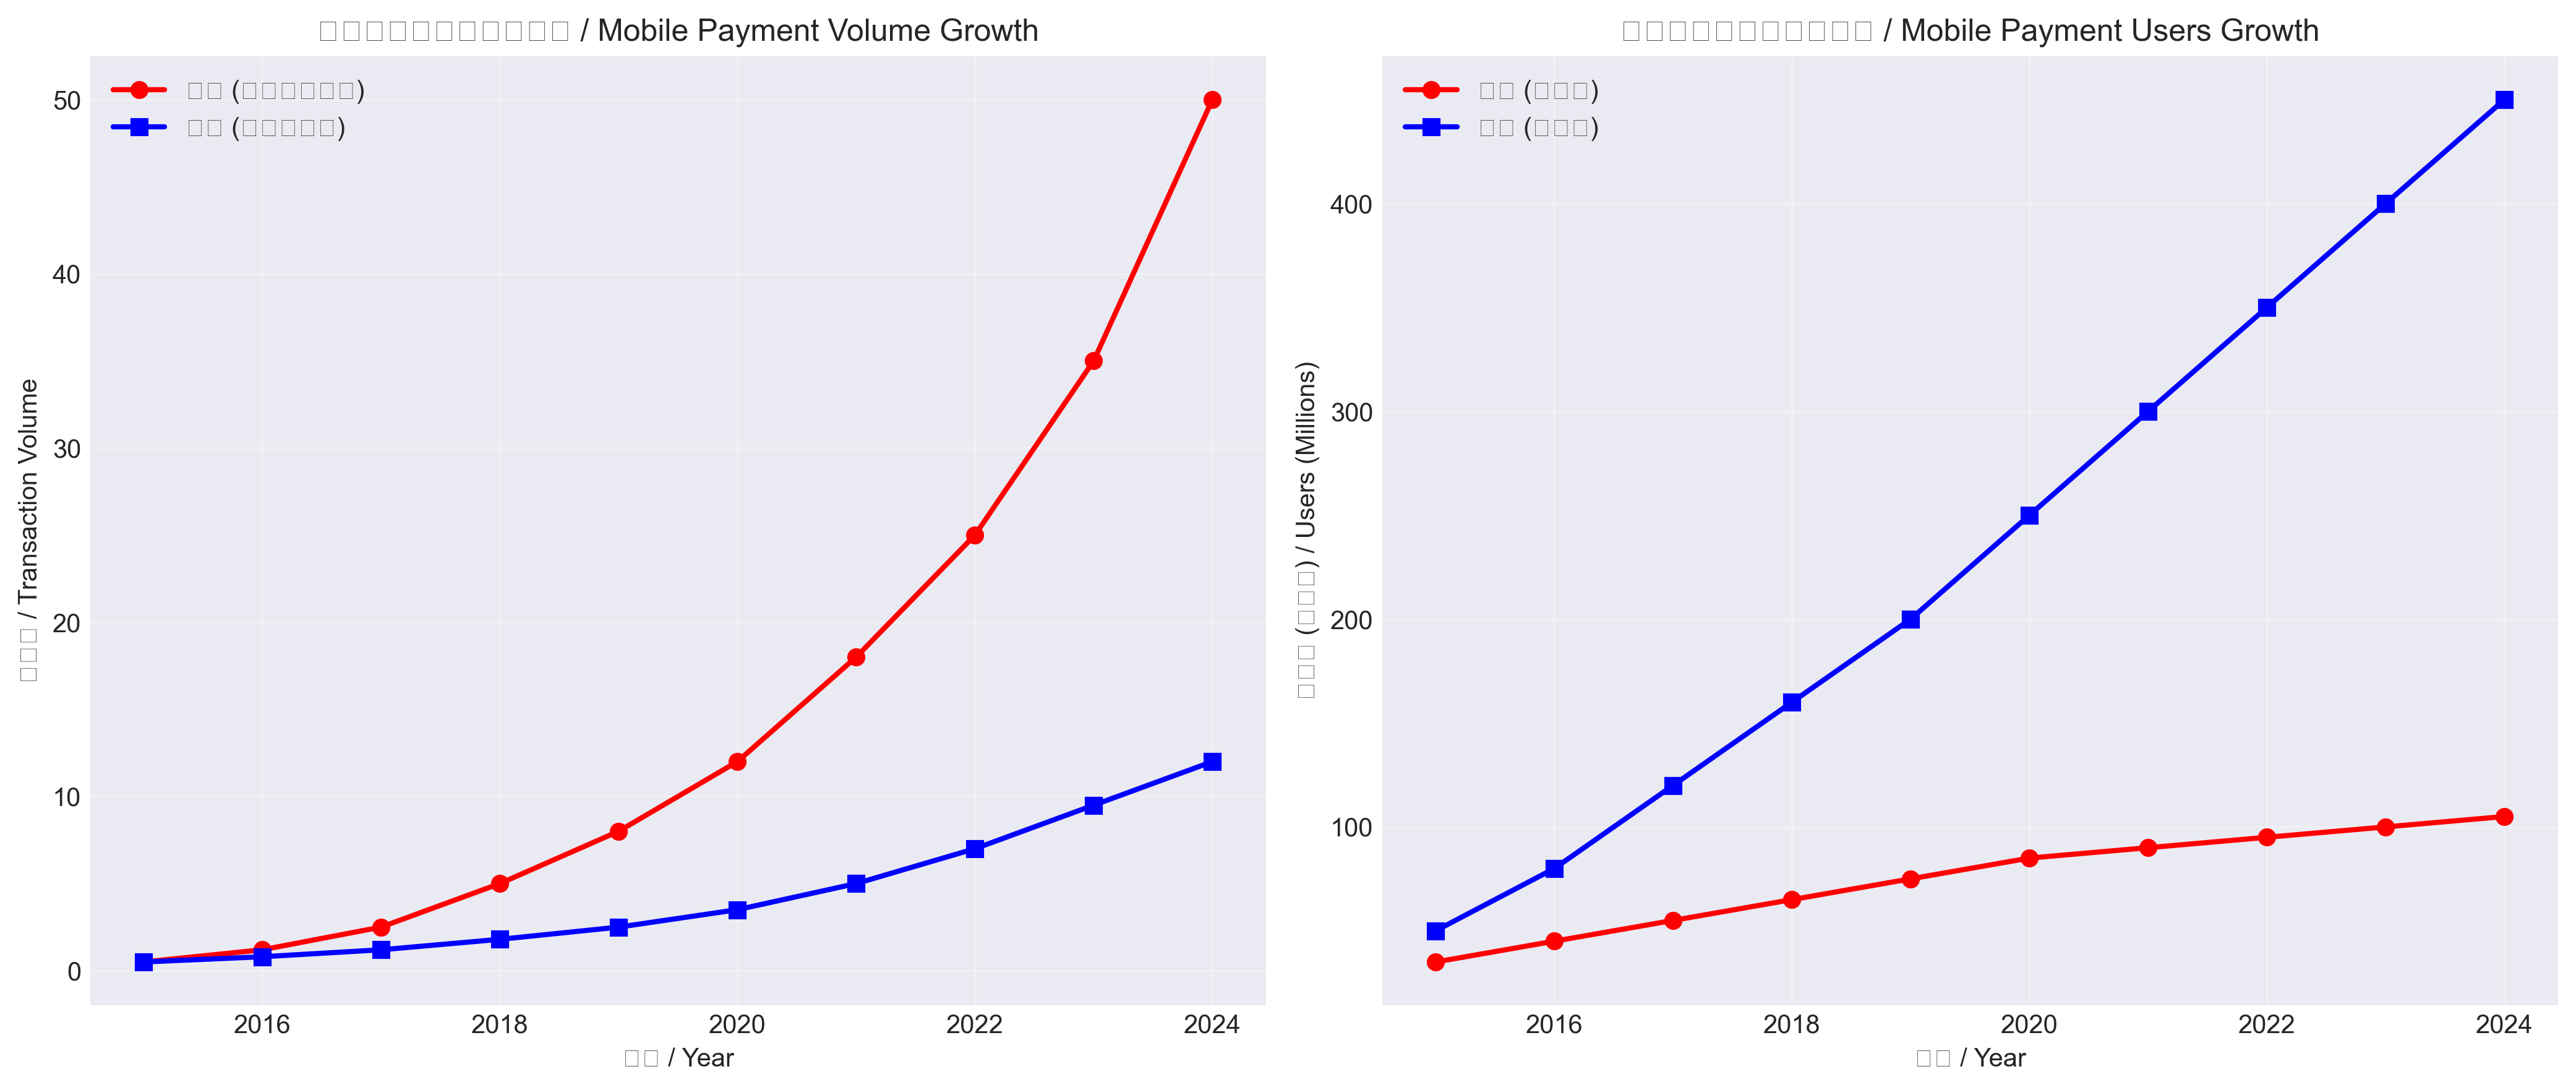
\includegraphics[width=0.9\textwidth]{figures/mobile_payment_growth.png}
\caption{Mobile Payment Growth Trends / Mobiles Zahlungswachstum-Trends}
\label{fig:payment-growth}
\end{figure}

如图~\ref{fig:payment-growth}所示，中国和欧洲在移动支付发展路径上存在显著差异。中国经历了爆发式增长，而欧洲的增长相对平缓，这反映了两个市场在支付基础设施成熟度上的根本差异。

As shown in Figure~\ref{fig:payment-growth}, there are significant differences in mobile payment development paths between China and Europe. China experienced explosive growth, while Europe's growth was relatively moderate, reflecting fundamental differences in payment infrastructure maturity between the two markets.

Wie in Abbildung~\ref{fig:payment-growth} dargestellt, gibt es erhebliche Unterschiede in den Entwicklungspfaden mobiler Zahlungen zwischen China und Europa. China erlebte ein explosives Wachstum, während Europas Wachstum relativ moderat war, was grundlegende Unterschiede in der Reife der Zahlungsinfrastruktur zwischen den beiden Märkten widerspiegelt.

\begin{itemize}
    
    \item \textbf{欧洲：渐进式演进}：欧洲经历了完整的支付技术演进（现金→支票→银行卡→电子支付），每个阶段都有成熟的解决方案，移动支付只是补充而非替代。
    \item \textbf{Europe: Gradual Evolution}: Europe experienced complete payment technology evolution (cash → checks → bank cards → electronic payments), with mature solutions at each stage. Mobile payments are complementary rather than replacements.
    \item \textbf{Europa: Graduelle Evolution}: Europa erlebte eine vollständige Zahlungstechnologie-Evolution (Bargeld → Schecks → Bankkarten → elektronische Zahlungen) mit reifen Lösungen in jeder Phase. Mobile Zahlungen sind ergänzend, nicht ersetzend.
    
    \item \textbf{基础设施成熟度}：欧洲的银行系统、支付网络（如SEPA）已经非常成熟，用户没有强烈的动机转向新的支付方式。
    \item \textbf{Infrastructure Maturity}: Europe's banking systems and payment networks (such as SEPA) are already very mature, and users have no strong motivation to switch to new payment methods.
    \item \textbf{Infrastrukturreife}: Europas Bankensysteme und Zahlungsnetzwerke (wie SEPA) sind bereits sehr reif, und Nutzer haben keine starke Motivation, zu neuen Zahlungsmethoden zu wechseln.
\end{itemize}

\subsection{互联网生态成熟度 / Internet Ecosystem Maturity / Reife des Internet-Ökosystems}

\textbf{不同的市场发展阶段 / Different Market Development Stages / Unterschiedliche Marktentwicklungsphasen}

\begin{itemize}
    \item \textbf{中国：移动优先的空白市场}：微信在中国兴起时（2011-2012年），移动互联网市场相对空白，为超级应用提供了发展空间。当时智能手机刚刚普及，用户对移动应用的需求旺盛。
    \item \textbf{China: Mobile-First Blank Market}: When WeChat emerged in China (2011-2012), the mobile internet market was relatively blank, providing development space for super apps. Smartphones had just become popular, and users had strong demand for mobile applications.
    \item \textbf{China: Mobile-First-Leermarkt}: Als WeChat in China entstand (2011-2012), war der mobile Internetmarkt relativ leer und bot Entwicklungsraum für Super-Apps. Smartphones waren gerade populär geworden, und Nutzer hatten starke Nachfrage nach mobilen Anwendungen.
    
    \item \textbf{欧洲：成熟的桌面互联网生态}：欧洲在移动互联网时代之前已有成熟的桌面互联网生态，用户习惯和商业模式已经建立，移动应用更多是现有服务的延伸。
    \item \textbf{Europe: Mature Desktop Internet Ecosystem}: Europe had a mature desktop internet ecosystem before the mobile internet era, with established user habits and business models. Mobile apps are more extensions of existing services.
    \item \textbf{Europa: Reifes Desktop-Internet-Ökosystem}: Europa hatte ein reifes Desktop-Internet-Ökosystem vor dem mobilen Internetzeitalter mit etablierten Nutzergewohnheiten und Geschäftsmodellen. Mobile Apps sind eher Erweiterungen bestehender Dienste.
    
    \item \textbf{平台竞争格局}：当微信试图进入欧洲时，Facebook、Google等平台已经建立了强大的移动生态，竞争格局已经形成。
    \item \textbf{Platform Competitive Landscape}: When WeChat attempted to enter Europe, platforms like Facebook and Google had already established strong mobile ecosystems, and the competitive landscape was already formed.
    \item \textbf{Plattform-Wettbewerbslandschaft}: Als WeChat versuchte, nach Europa zu kommen, hatten Plattformen wie Facebook und Google bereits starke mobile Ökosysteme etabliert, und die Wettbewerbslandschaft war bereits gebildet.
\end{itemize}

\section{商业模式差异 / Business Model Differences / Geschäftsmodellunterschiede}

\subsection{数据驱动的商业模式 / Data-Driven Business Models / Datengetriebene Geschäftsmodelle}

\textbf{数据收集与使用的限制 / Limitations on Data Collection and Use / Einschränkungen bei Datensammlung und -nutzung}

\begin{itemize}
    \item \textbf{中国模式}：微信通过收集用户行为数据，提供精准广告和推荐服务，这是其核心商业模式之一。微信可以从用户的聊天、支付、浏览等行为中提取数据，用于广告投放和商业决策。
    \item \textbf{Chinese Model}: WeChat collects user behavior data to provide precise advertising and recommendation services, which is one of its core business models. WeChat can extract data from users' chat, payment, browsing behaviors for advertising and business decisions.
    \item \textbf{Chinesisches Modell}: WeChat sammelt Nutzerverhaltensdaten, um präzise Werbung und Empfehlungsdienste bereitzustellen, was eines seiner Kern-Geschäftsmodelle ist. WeChat kann Daten aus Nutzer-Chat-, Zahlungs- und Browsing-Verhalten für Werbung und Geschäftsentscheidungen extrahieren.
    
    \item \textbf{欧洲限制}：GDPR严格限制数据收集和使用，要求明确的用户同意，禁止未经同意的数据共享。这严重限制了微信的数据驱动商业模式。根据GDPR，违反数据保护规定可能面临高达全球年营业额4\%或2000万欧元的罚款。
    \item \textbf{European Limitations}: GDPR strictly limits data collection and use, requiring explicit user consent and prohibiting unauthorized data sharing. This severely restricts WeChat's data-driven business model. Under GDPR, violations of data protection regulations can face fines of up to 4\% of global annual turnover or €20 million.
    \item \textbf{Europäische Einschränkungen}: Die DSGVO beschränkt Datensammlung und -nutzung streng, erfordert ausdrückliche Nutzereinwilligung und verbietet unautorisierte Datenweitergabe. Dies schränkt WeChats datengetriebenes Geschäftsmodell erheblich ein. Unter der DSGVO können Verstöße gegen Datenschutzbestimmungen Geldstrafen von bis zu 4\% des globalen Jahresumsatzes oder 20 Millionen Euro nach sich ziehen.
\end{itemize}

\begin{figure}[ht]
\centering
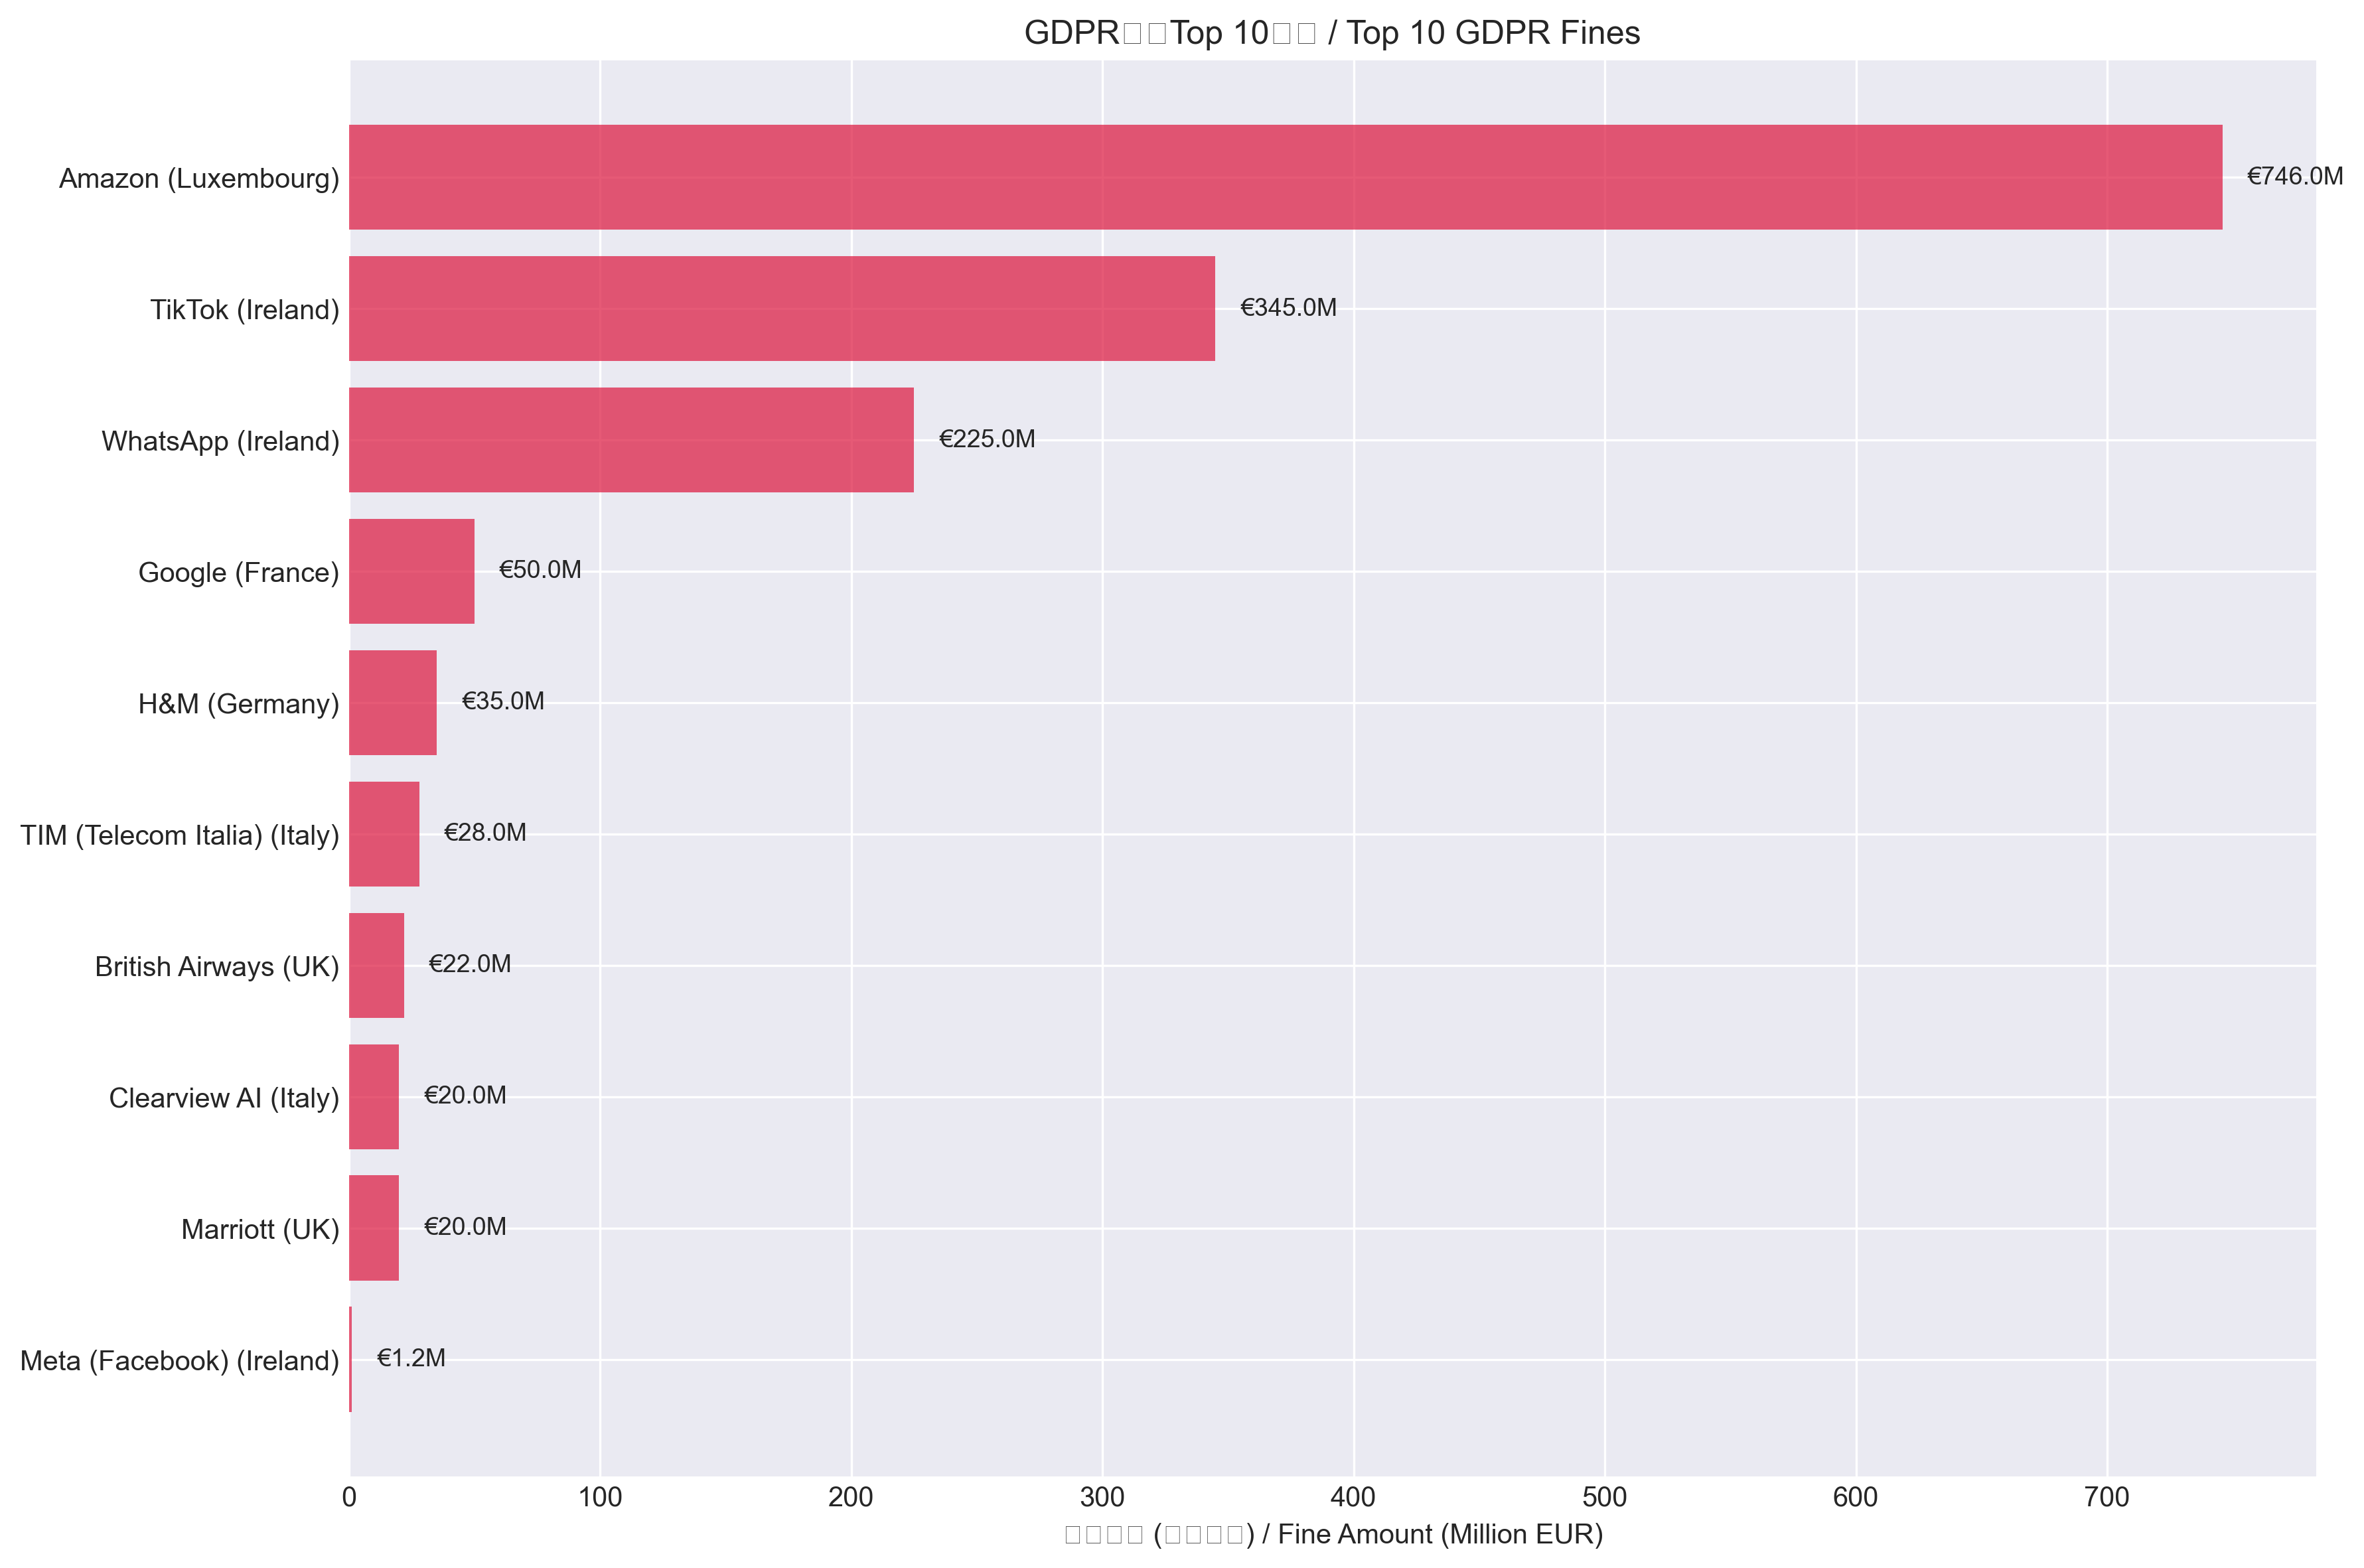
\includegraphics[width=0.9\textwidth]{figures/gdpr_fines_top10.png}
\caption{Top 10 GDPR Fines / Top 10 DSGVO-Geldstrafen}
\label{fig:gdpr-fines}
\end{figure}

如图~\ref{fig:gdpr-fines}所示，GDPR罚款案例显示了欧盟对数据保护违规行为的严格执法。最高罚款达到7.46亿欧元（Amazon, 2021年），这清楚地表明了GDPR合规的重要性。

As shown in Figure~\ref{fig:gdpr-fines}, GDPR fine cases demonstrate the EU's strict enforcement of data protection violations. The highest fine reached €746 million (Amazon, 2021), clearly demonstrating the importance of GDPR compliance.

Wie in Abbildung~\ref{fig:gdpr-fines} dargestellt, zeigen DSGVO-Geldstrafenfälle die strenge Durchsetzung von Datenschutzverstößen durch die EU. Die höchste Geldstrafe erreichte 746 Millionen Euro (Amazon, 2021), was deutlich die Bedeutung der DSGVO-Compliance zeigt.

\begin{itemize}
    
    \item \textbf{数据本地化要求}：一些欧洲国家要求数据存储在本地，这增加了微信的运营成本和复杂性。
    \item \textbf{Data Localization Requirements}: Some European countries require data to be stored locally, which increases WeChat's operational costs and complexity.
    \item \textbf{Datenlokalisierungsanforderungen}: Einige europäische Länder verlangen, dass Daten lokal gespeichert werden, was WeChats Betriebskosten und Komplexität erhöht.
\end{itemize}

\subsection{平台抽成模式 / Platform Commission Models / Plattform-Provisionsmodelle}

\textbf{不同的收入结构 / Different Revenue Structures / Unterschiedliche Einnahmestrukturen}

\begin{itemize}
    \item \textbf{微信模式}：通过整合多个服务，微信可以从支付、电商、广告等多个渠道获得收入，形成多元化的收入流。微信支付的交易手续费、小程序的服务费、广告收入等构成了其收入基础。
    \item \textbf{WeChat Model}: By integrating multiple services, WeChat can generate revenue from payments, e-commerce, advertising, and other channels, forming diversified revenue streams. WeChat Pay transaction fees, mini-program service fees, and advertising revenue form its income base.
    \item \textbf{WeChat-Modell}: Durch Integration mehrerer Dienste kann WeChat Einnahmen aus Zahlungen, E-Commerce, Werbung und anderen Kanälen generieren und vielfältige Einnahmequellen bilden. WeChat Pay-Transaktionsgebühren, Mini-Programm-Servicegebühren und Werbeeinnahmen bilden seine Einnahmebasis.
    
    \item \textbf{欧洲监管}：欧盟对平台抽成有更严格的监管，要求透明度和公平性，这可能限制微信的盈利模式。欧盟的数字服务法案（DSA）要求平台披露其算法和收费结构。
    \item \textbf{European Regulation}: The EU has stricter regulations on platform commissions, requiring transparency and fairness, which may limit WeChat's profit model. The EU's Digital Services Act (DSA) requires platforms to disclose their algorithms and fee structures.
    \item \textbf{Europäische Regulierung}: Die EU hat strengere Vorschriften für Plattformprovisionen, die Transparenz und Fairness erfordern, was WeChats Gewinnmodell einschränken könnte. Der Digital Services Act (DSA) der EU verlangt, dass Plattformen ihre Algorithmen und Gebührenstrukturen offenlegen.
    
    \item \textbf{反垄断审查}：欧盟对大型平台的抽成行为进行反垄断审查，可能要求降低费率或改变收费模式。
    \item \textbf{Antitrust Scrutiny}: The EU conducts antitrust scrutiny of large platforms' commission practices, potentially requiring fee reductions or changes to fee models.
    \item \textbf{Kartellrechtliche Prüfung}: Die EU führt kartellrechtliche Prüfungen der Provisionspraktiken großer Plattformen durch und könnte Gebührensenkungen oder Änderungen der Gebührenmodelle verlangen.
\end{itemize}

\section{本地化挑战 / Localization Challenges / Lokalisierungsherausforderungen}

\subsection{内容与文化适配 / Content and Cultural Adaptation / Inhalts- und kulturelle Anpassung}

\textbf{深度本地化的需求 / Need for Deep Localization / Bedarf an tiefer Lokalisierung}

\begin{itemize}
    \item \textbf{文化敏感性}：微信需要理解每个欧洲国家的文化、习俗、商业习惯，这需要大量的本地化投入。例如，德国的商业文化强调正式性、合同和书面协议，这与微信的"轻量级"商业模式可能不匹配。
    \item \textbf{Cultural Sensitivity}: WeChat needs to understand the culture, customs, and business practices of each European country, requiring substantial localization investment. For example, German business culture emphasizes formality, contracts, and written agreements, which may not match WeChat's "lightweight" business model.
    \item \textbf{Kulturelle Sensibilität}: WeChat muss die Kultur, Bräuche und Geschäftspraktiken jedes europäischen Landes verstehen, was erhebliche Lokalisierungsinvestitionen erfordert. Beispielsweise betont die deutsche Geschäftskultur Formalität, Verträge und schriftliche Vereinbarungen, was möglicherweise nicht zu WeChats "leichtgewichtigen" Geschäftsmodell passt.
    
    \item \textbf{内容审核}：不同国家对内容有不同的法律要求，微信需要为每个市场建立内容审核机制。例如，德国对仇恨言论有严格的法律，违反可能面临严重处罚。
    \item \textbf{Content Moderation}: Different countries have different legal requirements for content. WeChat needs to establish content moderation mechanisms for each market. For example, Germany has strict laws on hate speech, with violations potentially facing severe penalties.
    \item \textbf{Inhaltsmoderation}: Verschiedene Länder haben unterschiedliche rechtliche Anforderungen an Inhalte. WeChat muss Inhaltsmoderationsmechanismen für jeden Markt etablieren. Beispielsweise hat Deutschland strenge Gesetze gegen Hassrede, wobei Verstöße möglicherweise schwerwiegende Strafen nach sich ziehen.
    
    \item \textbf{语言本地化}：需要支持24种欧盟官方语言，每种语言都需要专业的翻译和本地化团队，成本极高。
    \item \textbf{Language Localization}: Need to support 24 EU official languages, each requiring professional translation and localization teams, with extremely high costs.
    \item \textbf{Sprachlokalisierung}: Notwendigkeit, 24 EU-Amtssprachen zu unterstützen, jede erfordert professionelle Übersetzungs- und Lokalisierungsteams mit extrem hohen Kosten.
\end{itemize}

\subsection{服务提供商网络 / Service Provider Networks / Dienstleisternetzwerke}

\textbf{建立本地合作伙伴关系的困难 / Difficulties in Establishing Local Partnerships / Schwierigkeiten beim Aufbau lokaler Partnerschaften}

\begin{itemize}
    \item \textbf{信任建立}：欧洲本地商家和服务提供商对来自中国的平台可能缺乏信任，建立合作关系需要时间。特别是在数据安全和隐私保护方面，欧洲商家可能担心与外国平台合作的风险。
    \item \textbf{Trust Building}: European local merchants and service providers may lack trust in platforms from China, requiring time to establish cooperative relationships. Particularly regarding data security and privacy protection, European merchants may worry about risks of partnering with foreign platforms.
    \item \textbf{Vertrauensaufbau}: Europäische lokale Händler und Dienstleister könnten Vertrauen in Plattformen aus China fehlen, was Zeit erfordert, um kooperative Beziehungen aufzubauen. Besonders in Bezug auf Datensicherheit und Datenschutz könnten europäische Händler sich Sorgen über Risiken der Partnerschaft mit ausländischen Plattformen machen.
    
    \item \textbf{竞争关系}：许多欧洲本地服务提供商可能将微信视为竞争对手而非合作伙伴。例如，欧洲的支付服务提供商可能担心微信支付会蚕食他们的市场份额。
    \item \textbf{Competitive Relationship}: Many European local service providers may view WeChat as a competitor rather than a partner. For example, European payment service providers may worry that WeChat Pay will erode their market share.
    \item \textbf{Wettbewerbsbeziehung}: Viele europäische lokale Dienstleister könnten WeChat als Wettbewerber und nicht als Partner betrachten. Beispielsweise könnten europäische Zahlungsdienstleister sich sorgen, dass WeChat Pay ihren Marktanteil erodiert.
    
    \item \textbf{商业文化差异}：欧洲的商业文化更强调合同、法律框架和正式协议，而微信的快速迭代、灵活合作的模式可能需要调整。
    \item \textbf{Business Culture Differences}: European business culture emphasizes contracts, legal frameworks, and formal agreements, while WeChat's rapid iteration and flexible cooperation model may need adjustment.
    \item \textbf{Geschäftskulturunterschiede}: Die europäische Geschäftskultur betont Verträge, Rechtsrahmen und formale Vereinbarungen, während WeChats Modell der schnellen Iteration und flexiblen Zusammenarbeit möglicherweise angepasst werden muss.
\end{itemize}

\section{总结与核心原因 / Summary and Core Reasons / Zusammenfassung und Kernursachen}

\subsection{五大核心原因 / Five Core Reasons / Fünf Kernursachen}

基于以上分析，微信生态模式在欧洲未能流行的根本原因可以归纳为以下五点：

Based on the above analysis, the fundamental reasons why WeChat's ecosystem model has not become popular in Europe can be summarized into the following five points:

Basierend auf der obigen Analyse können die grundlegenden Gründe, warum WeChats Ökosystemmodell in Europa nicht populär wurde, in die folgenden fünf Punkte zusammengefasst werden:

\begin{enumerate}
    \item \textbf{监管壁垒 / Regulatory Barriers / Regulatorische Barrieren}
    \begin{itemize}
        \item GDPR数据保护法规严格限制数据整合和跨服务数据共享
        \item GDPR data protection regulations strictly limit data integration and cross-service data sharing
        \item DSGVO-Datenschutzbestimmungen beschränken Datenintegration und dienstübergreifende Datenweitergabe streng
        \item 反垄断法规限制平台整合多个服务领域
        \item Antitrust regulations limit platforms' integration of multiple service areas
        \item Kartellrechtliche Vorschriften beschränken die Integration mehrerer Dienstbereiche durch Plattformen
        \item 金融监管要求获得复杂牌照，门槛高
        \item Financial regulations require obtaining complex licenses with high barriers
        \item Finanzvorschriften erfordern komplexe Lizenzen mit hohen Barrieren
    \end{itemize}
    
    \item \textbf{市场成熟度 / Market Maturity / Marktreife}
    \begin{itemize}
        \item 欧洲市场已被成熟平台占据（WhatsApp、PayPal、Amazon等）
        \item European markets are already occupied by mature platforms (WhatsApp, PayPal, Amazon, etc.)
        \item Europäische Märkte sind bereits von reifen Plattformen besetzt (WhatsApp, PayPal, Amazon, etc.)
        \item 用户习惯已形成，迁移成本高
        \item User habits are already formed with high switching costs
        \item Nutzergewohnheiten sind bereits gebildet mit hohen Wechselkosten
        \item 27+个独立市场需要分别本地化，成本极高
        \item 27+ independent markets require separate localization with extremely high costs
        \item 27+ unabhängige Märkte erfordern separate Lokalisierung mit extrem hohen Kosten
    \end{itemize}
    
    \item \textbf{用户行为差异 / User Behavior Differences / Unterschiede im Nutzerverhalten}
    \begin{itemize}
        \item 欧洲用户偏好功能分离的应用，而非超级应用
        \item European users prefer functionally separated apps rather than super apps
        \item Europäische Nutzer bevorzugen funktional getrennte Apps statt Super-Apps
        \item 对数据隐私有更强的意识和要求
        \item Have stronger awareness and requirements for data privacy
        \item Haben stärkeres Bewusstsein und Anforderungen für Datenschutz
        \item 习惯于多平台使用，而非单一平台集中
        \item Accustomed to multi-platform usage rather than single-platform concentration
        \item Gewohnt an Multi-Plattform-Nutzung statt Ein-Plattform-Konzentration
    \end{itemize}
    
    \item \textbf{基础设施差异 / Infrastructure Differences / Infrastrukturunterschiede}
    \begin{itemize}
        \item 欧洲已有成熟的银行卡和电子支付系统
        \item Europe already has mature bank card and electronic payment systems
        \item Europa hat bereits reife Bankkarten- und elektronische Zahlungssysteme
        \item 移动支付需求不如中国强烈
        \item Less urgent need for mobile payments than China
        \item Weniger dringender Bedarf an mobilen Zahlungen als China
        \item 成熟的桌面互联网生态已建立用户习惯
        \item Mature desktop internet ecosystem has already established user habits
        \item Reifes Desktop-Internet-Ökosystem hat bereits Nutzergewohnheiten etabliert
    \end{itemize}
    
    \item \textbf{文化价值观 / Cultural Values / Kulturelle Werte}
    \begin{itemize}
        \item 更强调个人数据主权和隐私保护
        \item Emphasize personal data sovereignty and privacy protection more
        \item Betonen persönliche Datensouveränität und Datenschutz stärker
        \item 偏好多元化选择，反对单一平台垄断
        \item Prefer diverse choices and oppose single-platform monopolies
        \item Bevorzugen vielfältige Auswahl und lehnen Ein-Plattform-Monopole ab
        \item 要求更高的透明度和用户控制权
        \item Require higher transparency and user control
        \item Erfordern höhere Transparenz und Nutzerkontrolle
    \end{itemize}
\end{enumerate}

\section{对德国创业地图平台的启示 / Insights for Germany Startup Map Platform / Erkenntnisse für die Germany Startup Map-Plattform}

\subsection{平台设计原则 / Platform Design Principles / Plattformdesignprinzipien}

基于微信在欧洲的经验教训，德国创业地图平台应该遵循以下设计原则：

Based on lessons from WeChat's experience in Europe, the Germany Startup Map platform should follow these design principles:

Basierend auf den Lehren aus WeChats Erfahrung in Europa sollte die Germany Startup Map-Plattform diese Designprinzipien befolgen:

\begin{enumerate}
    \item \textbf{合规优先设计 / Compliance-First Design / Compliance-First-Design}
    \begin{itemize}
        \item 从设计阶段就考虑GDPR合规，建立透明的数据使用政策
        \item Consider GDPR compliance from the design stage, establish transparent data usage policies
        \item DSGVO-Compliance bereits im Designstadium berücksichtigen, transparente Datennutzungsrichtlinien etablieren
        \item 实施数据最小化原则，只收集必要的数据
        \item Implement data minimization principles, collect only necessary data
        \item Datenminimierungsprinzipien implementieren, nur notwendige Daten sammeln
        \item 提供清晰的用户同意机制和数据控制选项
        \item Provide clear user consent mechanisms and data control options
        \item Klare Nutzereinwilligungsmechanismen und Datenkontrolloptionen bereitstellen
    \end{itemize}
    
    \item \textbf{模块化架构 / Modular Architecture / Modulare Architektur}
    \begin{itemize}
        \item 采用模块化设计，允许用户选择需要的服务，而非强制使用所有功能
        \item Adopt modular design, allowing users to choose needed services rather than forcing use of all features
        \item Modulares Design übernehmen, Nutzern ermöglichen, benötigte Dienste zu wählen, anstatt alle Funktionen zu erzwingen
        \item 每个模块可以独立使用，不依赖其他模块
        \item Each module can be used independently without depending on other modules
        \item Jedes Modul kann unabhängig verwendet werden, ohne von anderen Modulen abhängig zu sein
        \item 提供清晰的模块边界和数据隔离
        \item Provide clear module boundaries and data isolation
        \item Klare Modulgrenzen und Datenisolierung bereitstellen
    \end{itemize}
    
    \item \textbf{深度本地化 / Deep Localization / Tiefe Lokalisierung}
    \begin{itemize}
        \item 深度理解德国和欧洲市场的文化、法规、商业习惯
        \item Deeply understand the culture, regulations, and business practices of German and European markets
        \item Kultur, Vorschriften und Geschäftspraktiken deutscher und europäischer Märkte tief verstehen
        \item 提供德语、英语、中文三语支持
        \item Provide trilingual support (German, English, Chinese)
        \item Dreisprachige Unterstützung (Deutsch, Englisch, Chinesisch) bereitstellen
        \item 适配德国的商业文化和法律要求
        \item Adapt to German business culture and legal requirements
        \item An deutsche Geschäftskultur und rechtliche Anforderungen anpassen
    \end{itemize}
    
    \item \textbf{信任建立机制 / Trust-Building Mechanisms / Vertrauensaufbau-Mechanismen}
    \begin{itemize}
        \item 与本地服务提供商建立合作关系，而非竞争关系
        \item Establish cooperative relationships with local service providers rather than competitive ones
        \item Kooperative Beziehungen zu lokalen Dienstleistern aufbauen, nicht wettbewerbsorientierte
        \item 提供透明的服务条款和定价
        \item Provide transparent service terms and pricing
        \item Transparente Servicebedingungen und Preisgestaltung bereitstellen
        \item 建立用户评价和验证系统
        \item Establish user review and verification systems
        \item Nutzerbewertungs- und Verifizierungssysteme etablieren
    \end{itemize}
    
    \item \textbf{专业化定位 / Specialized Positioning / Spezialisierte Positionierung}
    \begin{itemize}
        \item 专注于中国企业家在德国的特定需求，而非试图成为"超级应用"
        \item Focus on specific needs of Chinese entrepreneurs in Germany, rather than attempting to become a "super app"
        \item Sich auf spezifische Bedürfnisse chinesischer Unternehmer in Deutschland konzentrieren, anstatt zu versuchen, eine "Super-App" zu werden
        \item 提供专业化的服务（商业信息、法律咨询、房地产数据、供应链连接）
        \item Provide specialized services (business information, legal consultation, real estate data, supply chain connections)
        \item Spezialisierte Dienste anbieten (Geschäftsinformationen, Rechtsberatung, Immobiliendaten, Lieferkettenverbindungen)
        \item 与现有平台互补，而非竞争
        \item Complement existing platforms rather than compete
        \item Bestehende Plattformen ergänzen, nicht konkurrieren
    \end{itemize}
\end{enumerate}

\subsection{差异化策略 / Differentiation Strategy / Differenzierungsstrategie}

\textbf{专注于特定需求 / Focus on Specific Needs / Fokus auf spezifische Bedürfnisse}

德国创业地图平台应该：

The Germany Startup Map platform should:

Die Germany Startup Map-Plattform sollte:

\begin{itemize}
    \item \textbf{垂直专业化}：专注于中国企业家在德国的创业需求，提供深度、专业的信息和服务，而非试图覆盖所有用户的所有需求。
    \item \textbf{Vertical Specialization}: Focus on the entrepreneurial needs of Chinese entrepreneurs in Germany, providing deep, professional information and services, rather than attempting to cover all needs of all users.
    \item \textbf{Vertikale Spezialisierung}: Sich auf die unternehmerischen Bedürfnisse chinesischer Unternehmer in Deutschland konzentrieren, tiefe, professionelle Informationen und Dienstleistungen bereitstellen, anstatt zu versuchen, alle Bedürfnisse aller Nutzer abzudecken.
    
    \item \textbf{桥梁作用}：作为连接中国企业家与德国资源的桥梁，而非试图替代现有服务。
    \item \textbf{Bridge Role}: Act as a bridge connecting Chinese entrepreneurs with German resources, rather than attempting to replace existing services.
    \item \textbf{Brückenfunktion}: Als Brücke fungieren, die chinesische Unternehmer mit deutschen Ressourcen verbindet, anstatt zu versuchen, bestehende Dienste zu ersetzen.
    
    \item \textbf{价值创造}：通过减少信息不对称、降低交易成本、提供专业指导来创造价值，而非通过数据垄断。
    \item \textbf{Value Creation}: Create value by reducing information asymmetry, lowering transaction costs, and providing professional guidance, rather than through data monopoly.
    \item \textbf{Wertschöpfung}: Wert schaffen durch Reduzierung von Informationsasymmetrie, Senkung von Transaktionskosten und Bereitstellung professioneller Anleitung, nicht durch Datenmonopol.
\end{itemize}

\section{结论 / Conclusion / Fazit}

微信生态模式在欧洲未能流行的根本原因在于：欧洲的监管环境、市场成熟度、用户习惯、基础设施和文化价值观与微信成功所需的条件存在根本性差异。这些差异不是技术问题，而是深层次的结构性、文化性和制度性差异。

The fundamental reason why WeChat's ecosystem model has not become popular in Europe lies in: fundamental differences between Europe's regulatory environment, market maturity, user habits, infrastructure, and cultural values and the conditions needed for WeChat's success. These differences are not technical issues but deep-seated structural, cultural, and institutional differences.

Der grundlegende Grund, warum WeChats Ökosystemmodell in Europa nicht populär wurde, liegt in: grundlegenden Unterschieden zwischen Europas regulatorischem Umfeld, Marktreife, Nutzergewohnheiten, Infrastruktur und kulturellen Werten und den Bedingungen, die für WeChats Erfolg benötigt werden. Diese Unterschiede sind keine technischen Probleme, sondern tief verwurzelte strukturelle, kulturelle und institutionelle Unterschiede.

对于德国创业地图平台而言，关键启示是：**不要试图复制微信的超级应用模式，而是要专注于特定需求，提供专业化、合规化、本地化的服务，与现有生态系统互补而非竞争。**

For the Germany Startup Map platform, the key insight is: **Don't attempt to replicate WeChat's super-app model, but instead focus on specific needs, provide specialized, compliant, localized services, complementing rather than competing with existing ecosystems.**

Für die Germany Startup Map-Plattform ist die wichtige Erkenntnis: **Versuchen Sie nicht, WeChats Super-App-Modell zu replizieren, sondern konzentrieren Sie sich auf spezifische Bedürfnisse, bieten Sie spezialisierte, konforme, lokalisierte Dienstleistungen an, die bestehende Ökosysteme ergänzen, anstatt mit ihnen zu konkurrieren.**

\end{document}
